\documentclass[UTF8]{ctexart}
\usepackage{amsmath}
\usepackage{amssymb}
\usepackage{xparse,tikz}
\usetikzlibrary{calc}
\usepackage[margin=2cm]{geometry}
\usepackage{graphicx}
\usepackage{zhnumber}
\usepackage{float}
\usepackage{booktabs}
\usepackage{subcaption}
\usepackage{array}
\usepackage{caption}
\captionsetup{font=small}

\newcommand{\Zzero}{Z_0}
\newcommand{\dd}{\mathrm{d}}
\renewcommand{\arraystretch}{1.18}

\NewDocumentCommand{\drawsmithchart}{}
{
  \begin{tikzpicture}[x=3.15cm,y=3.15cm,>=stealth]
    \begin{scope}
      \clip (0,0) circle (1);
      \foreach \r in {0.2,0.5,1,2,5}
      {
        \draw[gray!45,thin] ({\r/(1+\r)},0) circle ({1/(1+\r)});
      }
      \foreach \x in {0.2,0.5,1,2,5,-0.2,-0.5,-1,-2,-5}
      {
        \draw[gray!45,thin] (1,{1/\x}) circle ({abs(1/\x)});
      }
      \draw[red!60,dashed,thick] (0,0) circle (0.5312);
    \end{scope}
    \draw[black,thick] (0,0) circle (1);
    \draw[black!65,thin] (-1,0) -- (1,0);
    \draw[black!65,thin] (0,-1) -- (0,1);
    \foreach \r/\lab in {0.2/0.2,0.5/0.5,1/1,2/2,5/5}
    {
      \node[gray!70,font=\scriptsize] at ({(\r-1)/(\r+1)},0.035) {$r=\lab$};
    }
    \node[font=\scriptsize] at (0,0.09) {匹配};
    \node[font=\scriptsize,anchor=east] at (-1.02,0) {短路};
    \node[font=\scriptsize,anchor=west] at (1.02,0) {开路};
    \draw[red!65,dashed] (0,0) -- (-0.4306,-0.3110);
    \fill[red!85!black] (-0.4306,-0.3110) circle (0.018);
    \node[red!85!black,font=\small,anchor=north east] at (-0.4306,-0.3110)
      {$\Gamma_L$};
    \draw[red!85!black,->,thick] (-0.10,-0.18) -- (-0.410,-0.296);
    \node[align=left,font=\scriptsize,anchor=west,text width=4.1cm] at (1.18,-0.42)
    {
      $|\Gamma_L|=0.5312$\\
      $\angle\Gamma_L=-144.16^\circ$\\
      $z_L=0.3349-j0.2902$\\
      $\rho=3.266$
    };
    \node[red!70,font=\scriptsize,anchor=west] at (0.40,0.58)
      {等驻波系数圆};
  \end{tikzpicture}
}

\NewDocumentCommand{\drawadmittancematchchart}{}
{
  \begin{tikzpicture}[x=3.05cm,y=3.05cm,>=stealth]
    \begin{scope}
      \clip (0,0) circle (1);
      \foreach \g in {0.2,0.5,1,2,5}
      {
        \draw[gray!45,thin] ({\g/(1+\g)},0) circle ({1/(1+\g)});
      }
      \foreach \b in {0.2,0.5,1,2,5,-0.2,-0.5,-1,-2,-5}
      {
        \draw[gray!45,thin] (1,{1/\b}) circle ({abs(1/\b)});
      }
      \draw[blue!55,dashed,thick] (0,0) circle (0.5312);
      \draw[blue!70,->,thick] (35.85:0.5312) arc (35.85:-58.65:0.5312);
    \end{scope}
    \draw[black,thick] (0,0) circle (1);
    \draw[black!65,thin] (-1,0) -- (1,0);
    \draw[black!65,thin] (0,-1) -- (0,1);
    \foreach \g/\lab in {0.2/0.2,0.5/0.5,1/1,2/2,5/5}
    {
      \node[gray!70,font=\scriptsize] at ({(\g-1)/(\g+1)},0.035) {$g=\lab$};
    }
    \fill[blue!75!black] (0.4306,0.3110) circle (0.018);
    \node[blue!75!black,font=\small,anchor=south west] at (0.4306,0.3110)
      {$y_L$};
    \fill[orange!90!black] (0.2764,-0.4537) circle (0.018);
    \node[orange!90!black,font=\small,anchor=north west] at (0.2764,-0.4537)
      {$y(l)$};
    \fill[green!45!black] (0,0) circle (0.018);
    \node[green!45!black,font=\small,anchor=south east] at (-0.02,0.02)
      {$1+j0$};
    \draw[orange!90!black,->,thick] (0.2764,-0.4537) -- (0.015,-0.015);
    \node[orange!90!black,font=\scriptsize,anchor=west,text width=3.4cm] at (0.55,-0.52)
      {并联销钉\\$+j1.25$};
    \node[blue!70,font=\scriptsize,anchor=west,text width=3.6cm] at (0.48,0.56)
      {沿波导移动\\$l_\mathrm{eff}=0.580\,\mathrm{cm}$};
    \node[align=left,font=\scriptsize,anchor=west,text width=4.4cm] at (1.18,0.03)
    {
      $y_L=1.7055+j1.4777$\\
      $y(l)=0.984-j1.244$\\
      $y(l)+y_\mathrm{pin}\approx1+j0$
    };
    \node[font=\scriptsize,anchor=east] at (-1.02,0) {开路};
    \node[font=\scriptsize,anchor=west] at (1.02,0) {短路};
  \end{tikzpicture}
}

\NewDocumentCommand{\makecover}{}{
  \begin{titlepage}
  \begin{center}
  \vspace*{5cm}
  {\LARGE\bfseries 电磁场与电磁波}\par
  \vspace{1.5cm}
  {\Large\bfseries 波导传输线负载测量与阻抗匹配}\par
  \vspace{1cm}
  {\large 实验报告}
  \end{center}
  \end{titlepage}
}

\NewDocumentCommand{\makecoveri}{}{
  \begin{center}
  \begin{minipage}[c][145pt][c]{\textwidth}
  \centering{\Large\bfseries 电磁场与电磁波}\par
  \vspace{1cm}
  {\large 波导传输线负载测量与阻抗匹配}
  \end{minipage}
  \end{center}
}

\newcounter{makepart}
\setcounter{makepart}{1}
\NewDocumentCommand{\makepart}{+m}
{
  \vspace{1em}
  \begin{flushleft}
   \large\bfseries\zhnumber{\arabic{makepart}}、#1
  \end{flushleft}
  \stepcounter{makepart}
}

\NewDocumentCommand{\zdx}{}
{
  \tikz[remember picture,overlay]{
    \coordinate (s) at ([shift={(1,-3)}]current page.north west);
    \coordinate (e) at ([shift={(1,3)}]current page.south west);
    \foreach \x in{0,0.15,...,9.2}
    {
      \fill[] ($(s)+(0,-\x)$) circle(1pt);
    }
    \foreach \x in{0,0.15,...,9.2}
    {
      \fill[] ($(e)+(0,\x)$) circle(1pt);
    }
    \node[text width=1em,align=center]at($(s)!0.5!(e)$){装\\[10pt]订\\[10pt]线};
  }
}

\pagestyle{empty}

\begin{document}
\makecover
\makecoveri
\zdx

\section{实验目的与任务}

\subsection{实验目的}

本实验围绕矩形波导传输线的负载测量与阻抗匹配展开。通过驻波测量线、频率计、定向耦合器、检波器和单销钉调配器等微波部件，掌握波导工作频率、波导波长、负载反射系数、驻波系数和归一化阻抗的测量与换算方法。实验重点是将波导中的驻波分布与传输线等效模型相联系，并观察容性膜片负载在未匹配与经单销钉调配后的反射状态变化。

\subsection{实验任务}

\begin{enumerate}
  \item 搭建矩形波导负载测量系统，读出固态微波信号源的工作频率。
  \item 在短路终端条件下测量相邻波节点位置，计算实测波导波长，并与 TE$_{10}$ 模理论值比较。
  \item 测量容性膜片加匹配负载时的驻波最大、最小读数，求驻波系数、反射系数、归一化阻抗和归一化导纳。
  \item 使用单销钉调配器对容性膜片负载进行匹配，比较调配前、调配后和直接接匹配负载时的驻波系数。
  \item 根据销钉到负载的距离，估算匹配状态下销钉需要提供的归一化电纳，并用 Smith 圆图思想解释匹配机理。
  \item 回答实验指导书中的思考题，并结合实测过程分析误差来源。
\end{enumerate}

\subsection{实验仪器与元件}

\begin{table}[H]
  \centering
  \caption{实验所用主要仪器与波导元件}
  \label{tab:instrument}
  \begin{tabular}{ll}
    \toprule
    类别 & 名称与用途 \\
    \midrule
    信号与保护部件 & 固态微波信号源、隔离器、可调衰减器 \\
    测量部件 & 直读式频率计、驻波测量线、波导检波器、数字万用表、示波器 \\
    波导网络部件 & 反接定向耦合器、短路块、容性膜片、匹配负载、单销钉调配器 \\
    基本尺寸 & 矩形波导宽边 $a=2.286\,\mathrm{cm}$，窄边 $b=1.016\,\mathrm{cm}$ \\
    \bottomrule
  \end{tabular}
\end{table}

实验数据由小组共同采集，本文对记录数据进行独立整理、计算和讨论。测量系统连接示意见图 \ref{fig:system}，其中定向耦合器用于对反射功率取样，驻波测量线用于沿波导纵向寻找场强极值点。

\begin{figure}[H]
  \centering
  \begin{subfigure}{0.48\textwidth}
    \centering
    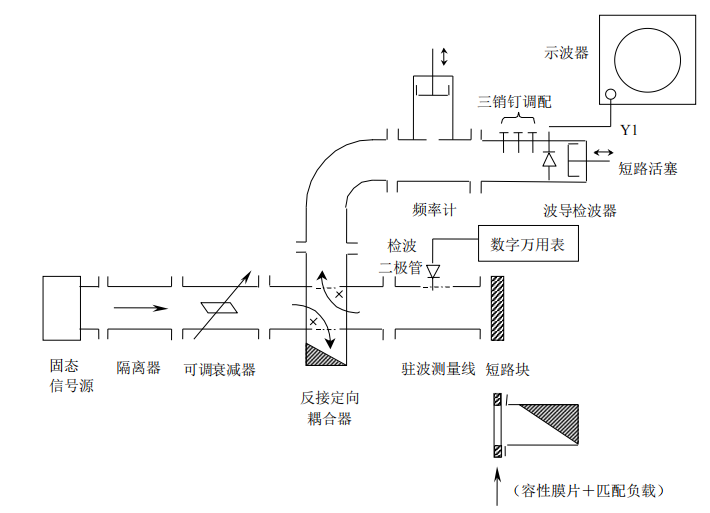
\includegraphics[width=\textwidth]{figures/measurement_system.png}
    \caption{负载测量系统}
  \end{subfigure}
  \begin{subfigure}{0.48\textwidth}
    \centering
    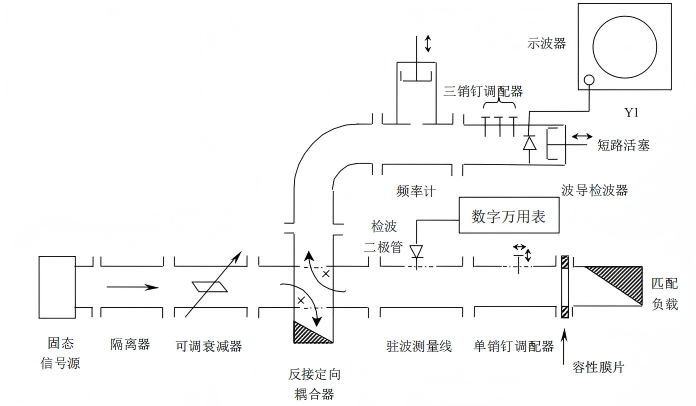
\includegraphics[width=\textwidth]{figures/matching_system.png}
    \caption{加入单销钉调配器的系统}
  \end{subfigure}
  \caption{波导负载测量与阻抗匹配实验连接示意}
  \label{fig:system}
\end{figure}

\section{实验原理}

\subsection{波导的传输线等效}

纵向均匀的金属波导中，某一确定模式的横向场分量可写成横向模式函数与沿传播方向变化的幅值相乘的形式。对 TE 或 TM 模而言，可记为
\begin{equation}
  \mathbf{E}_t=\mathbf{e}(\rho)V(z),\qquad
  \mathbf{H}_t=\mathbf{h}(\rho)I(z).
\end{equation}
其中 $V(z)$ 与 $I(z)$ 并不是低频意义下的端电压和端电流，而是描述横向电、磁场幅值沿 $z$ 方向变化的等效量。它们满足形式上类似传输线方程的关系：
\begin{equation}
  \frac{\dd V}{\dd z}=-jk_zZI,\qquad
  \frac{\dd I}{\dd z}=-jk_zYV.
  \label{eq:tl-equation}
\end{equation}
传播常数满足
\begin{equation}
  k_z^2=k^2-k_t^2,\qquad k=\omega\sqrt{\mu\varepsilon},
\end{equation}
而等效波阻抗与模式类型有关。对本实验的矩形波导 TE$_{10}$ 主模，有
\begin{equation}
  Z_\mathrm{TE}=\frac{\omega\mu}{k_z}.
\end{equation}
因此，在只激励 TE$_{10}$ 模且高次模截止的频段内，矩形波导可以被看作具有特定传播常数和特性阻抗的传输线。该等效关系是用驻波分布反推负载特性的基础。

\subsection{驻波系数与反射系数}

若波导终端负载与传输线特性阻抗不相等，入射波在负载处发生反射。沿线电场幅值由入射波和反射波叠加，形成如图 \ref{fig:standing-wave} 所示的驻波分布。驻波系数定义为
\begin{equation}
  \rho=\frac{V_{\max}}{V_{\min}}
       =\frac{1+|\Gamma|}{1-|\Gamma|},
  \label{eq:vswr}
\end{equation}
由此可反解反射系数幅值：
\begin{equation}
  |\Gamma|=\frac{\rho-1}{\rho+1}.
  \label{eq:gamma-mag}
\end{equation}
本实验中万用表读出的是检波输出。探针插入较浅、检波二极管处于小信号平方律区时，万用表读数可看作与相对功率成正比。因此驻波系数按
\begin{equation}
  \rho=\sqrt{\frac{P_{\max}}{P_{\min}}}
  \label{eq:rho-power}
\end{equation}
计算，其中 $P_{\max}$ 与 $P_{\min}$ 分别为波腹和波节点处的万用表读数。

\begin{figure}[H]
  \centering
  \begin{subfigure}{0.45\textwidth}
    \centering
    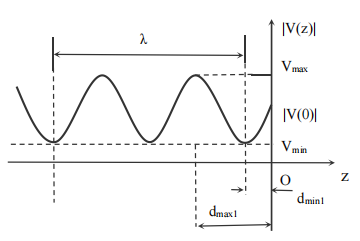
\includegraphics[width=0.95\textwidth]{figures/standing_wave.png}
    \caption{驻波幅值分布}
  \end{subfigure}
  \begin{subfigure}{0.45\textwidth}
    \centering
    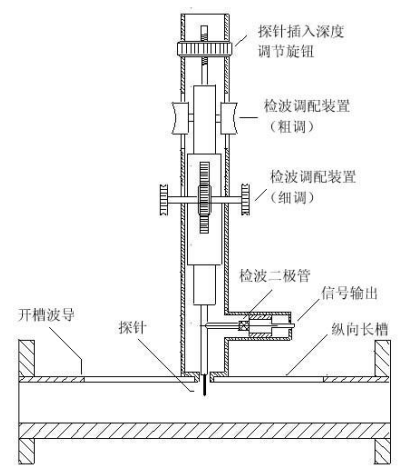
\includegraphics[width=0.95\textwidth]{figures/slotted_line.png}
    \caption{驻波测量线结构}
  \end{subfigure}
  \caption{驻波测量线读数的物理含义}
  \label{fig:standing-wave}
\end{figure}

\subsection{波导波长}

当波导终端接短路块时，负载反射系数幅值接近 1，沿线形成明显的纯驻波。相邻两个电压最小点相距半个波导波长，因此
\begin{equation}
  \lambda_{g,\mathrm{exp}}=2|d_{\min2}-d_{\min1}|.
  \label{eq:lambdag-exp}
\end{equation}
另一方面，矩形波导 TE$_{10}$ 模的截止波长为 $\lambda_c=2a$，自由空间波长为
\begin{equation}
  \lambda_0=\frac{c}{f}.
\end{equation}
理论波导波长为
\begin{equation}
  \lambda_{g,\mathrm{th}}
  =\frac{\lambda_0}
  {\sqrt{1-(\lambda_0/\lambda_c)^2}}
  =\frac{\lambda_0}
  {\sqrt{1-(\lambda_0/2a)^2}}.
  \label{eq:lambdag-th}
\end{equation}
由于 $\lambda_g$ 随频率变化显著，频率计读数误差会直接传递到理论值比较中。

\subsection{负载阻抗与驻波相位}

反射系数与归一化负载阻抗 $z_L=Z_L/\Zzero$ 的关系为
\begin{equation}
  z_L=\frac{1+\Gamma_L}{1-\Gamma_L},\qquad
  y_L=\frac{1}{z_L}.
  \label{eq:z-y}
\end{equation}
其中 $y_L$ 为归一化导纳。要确定 $\Gamma_L$ 的相位，仅有驻波系数还不够，还需知道第一个波节点相对参考面的移动量。本实验先测短路块条件下的波节点位置 $d_{\min}(\text{短})$，再测接入容性膜片后的波节点位置 $d_{\min}(\text{膜片})$，由两者的相对位移得到负载相位：
\begin{equation}
  \Delta d=d_{\min}(\text{短})-d_{\min}(\text{膜片}),
  \qquad
  \varphi_L=4\pi\left(\frac{\Delta d}{\lambda_g}-\frac{1}{4}\right).
  \label{eq:phase}
\end{equation}
这样可以消除测量线刻度零点、法兰面位置和短路块等效短路面带来的共同偏移。

容性膜片可看作在波导横截面处引入的并联容性电纳。若以导纳形式表示，其典型特征是
\begin{equation}
  y_L=g_L+jb_L,\qquad b_L>0.
  \label{eq:capacitive}
\end{equation}
也就是说，容性膜片在阻抗圆图上表现为负电抗，在导纳圆图上表现为正电纳。

\subsection{单销钉阻抗匹配}

单销钉调配器相当于在波导某一截面并联一个可调电纳。设从负载向信号源方向移动距离 $l$ 后的归一化导纳为
\begin{equation}
  y(l)=\frac{y_L+j\tan(\beta l)}
            {1+jy_L\tan(\beta l)},\qquad
  \beta=\frac{2\pi}{\lambda_g}.
  \label{eq:y-transform}
\end{equation}
若选择合适的销钉位置，使该截面处的实部接近 1，即
\begin{equation}
  y(l)\approx 1+jb,
\end{equation}
再调节销钉插入深度提供
\begin{equation}
  y_\mathrm{pin}\approx -jb,
  \label{eq:pin}
\end{equation}
则总归一化导纳接近 $1+j0$，从信号源侧看进去即达到匹配。Smith 圆图上，这一过程可理解为先沿等驻波系数圆旋转到 $g=1$ 圆，再用并联电纳把点移动到圆心。

\section{实验过程}

\subsection{工作频率测量}

实验开始时，测量线开口端接短路块，信号源设置为方波调制。调节波导检波器中的短路活塞和三销钉调配器，使示波器上的检波方波幅度较大且稳定。随后缓慢调节直读式频率计，当频率计谐振吸收能量时，示波器上的方波幅度出现明显下降，此时频率计刻度即为系统工作频率。实验照片如图 \ref{fig:freq-photo} 所示，读得
\[
  f=9.376\,\mathrm{GHz}.
\]

\begin{figure}[H]
  \centering
  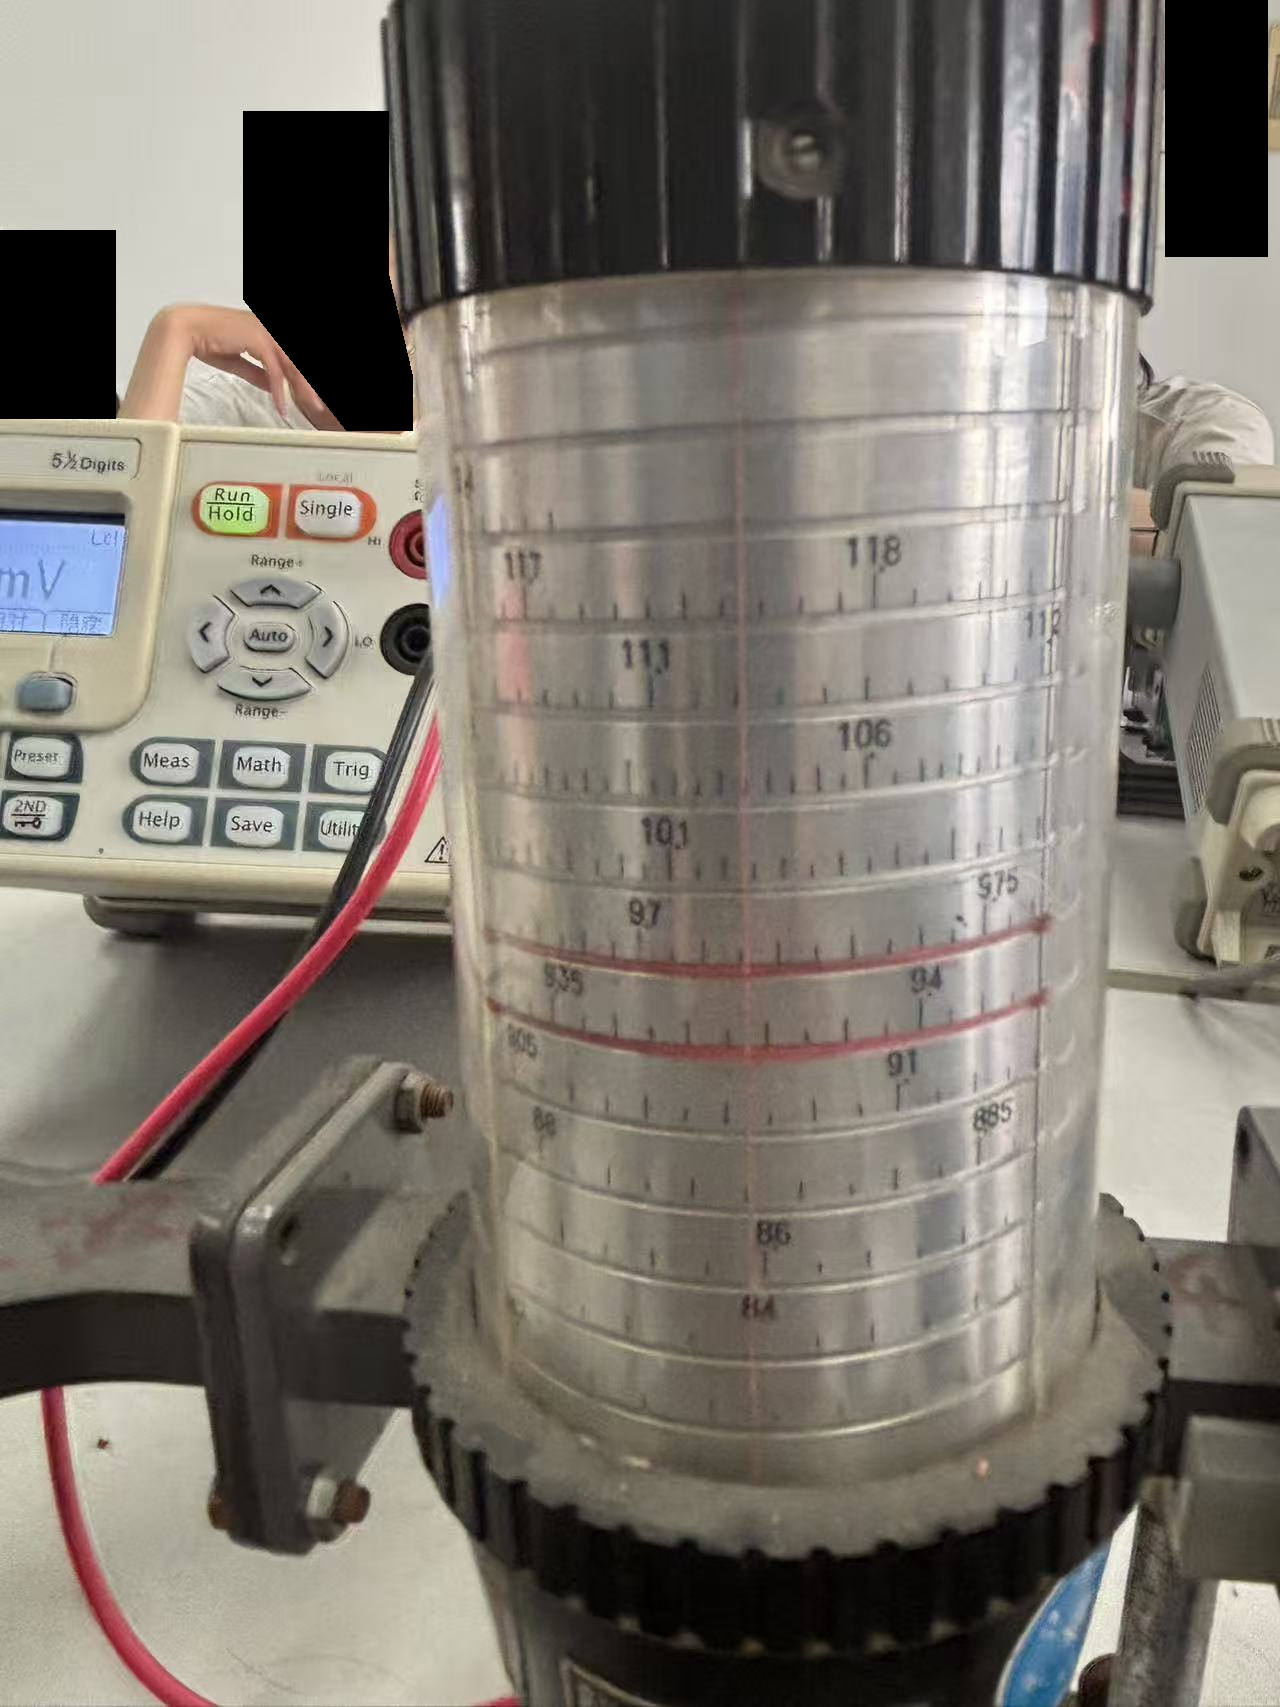
\includegraphics[width=0.62\textwidth]{figures/work_frequency.png}
  \caption{工作频率测量时的频率计读数}
  \label{fig:freq-photo}
\end{figure}

\subsection{波导波长测量}

保持短路块接入，使终端近似全反射。将驻波测量线探针插入约 $1\,\mathrm{mm}$，并调节检波匹配。先将探针移动到波腹附近，调节衰减器使万用表读数约为 $0.500\,\mathrm{mV}$，记录衰减器刻度。随后沿测量线缓慢移动探针，寻找相邻两个波节点位置。该过程的衰减器设置和波节点读数见图 \ref{fig:wavelength-photo}。

\begin{figure}[H]
  \centering
  \begin{subfigure}{0.32\textwidth}
    \centering
    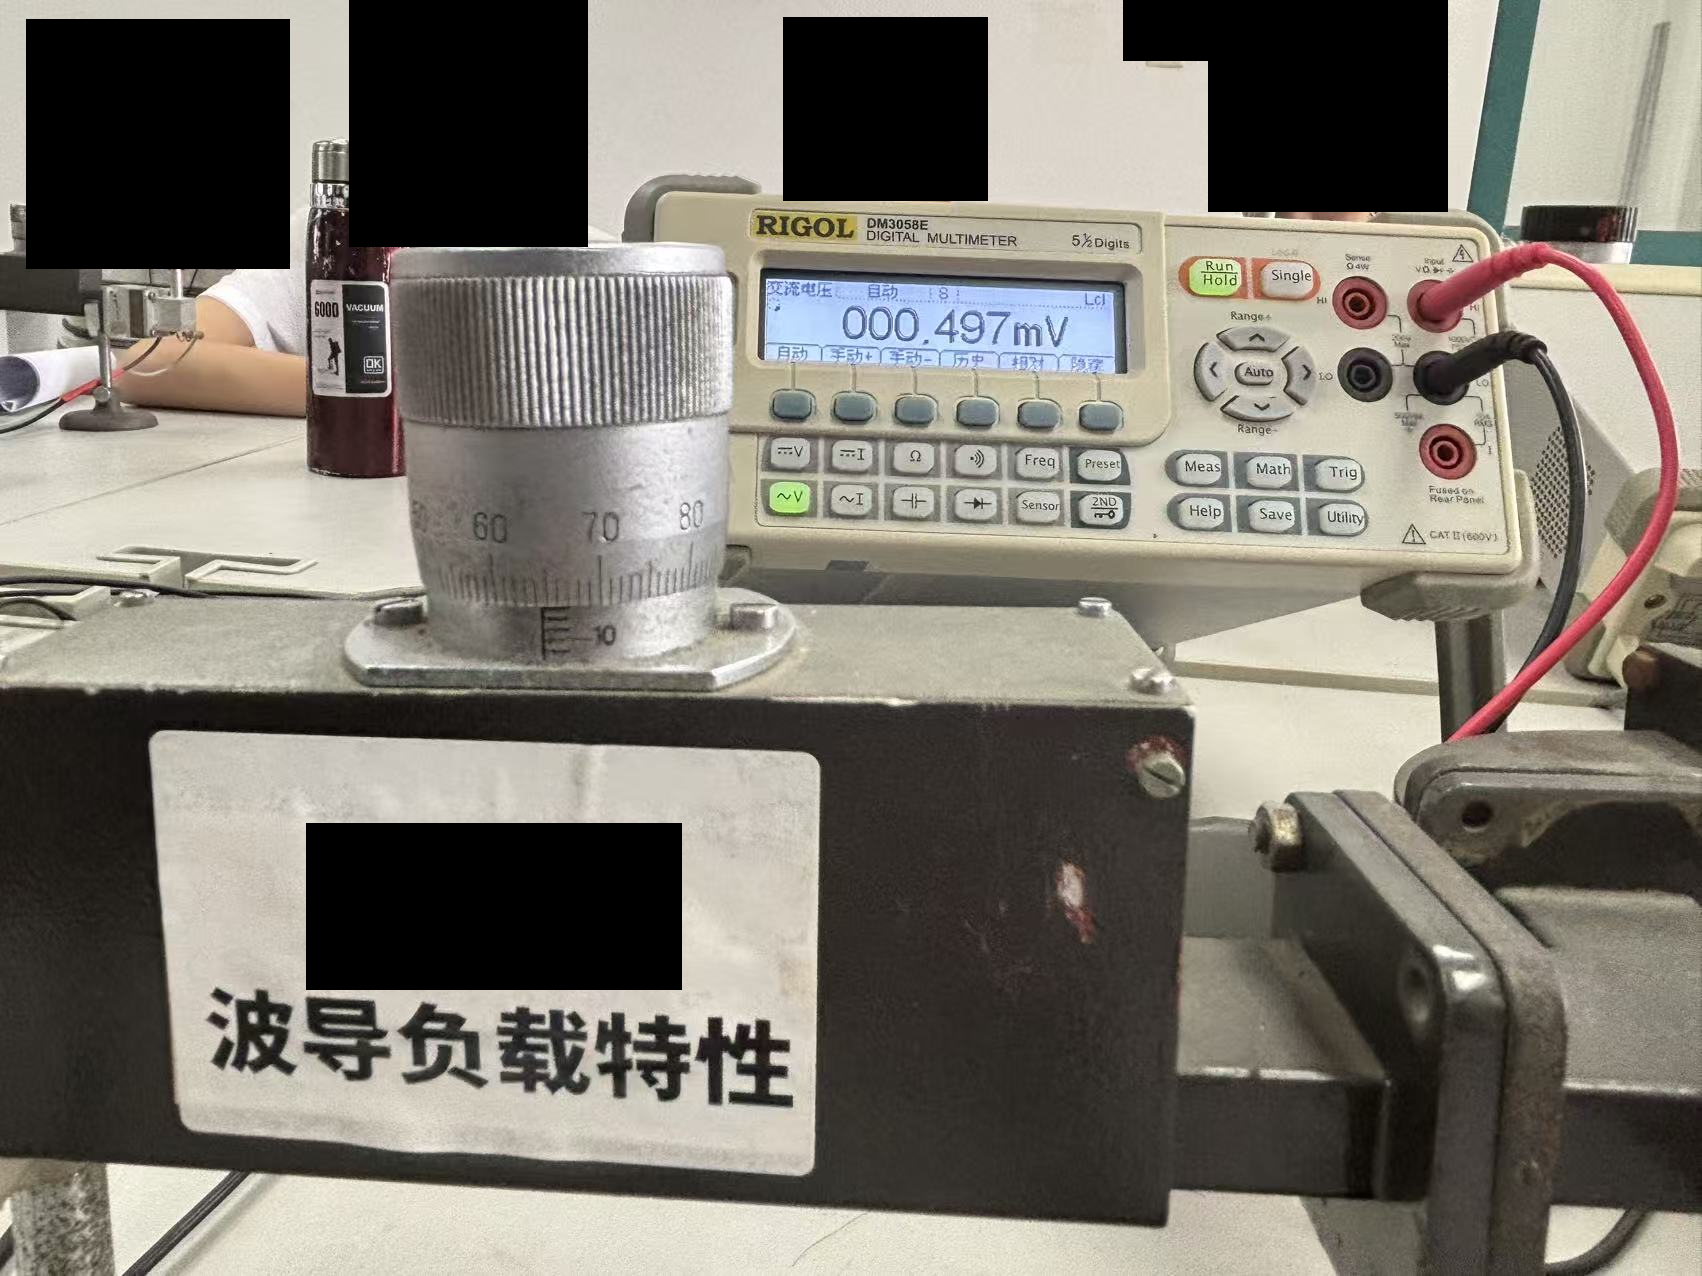
\includegraphics[width=\textwidth]{figures/attenuator_wavelength.png}
    \caption{调节衰减器}
  \end{subfigure}
  \begin{subfigure}{0.32\textwidth}
    \centering
    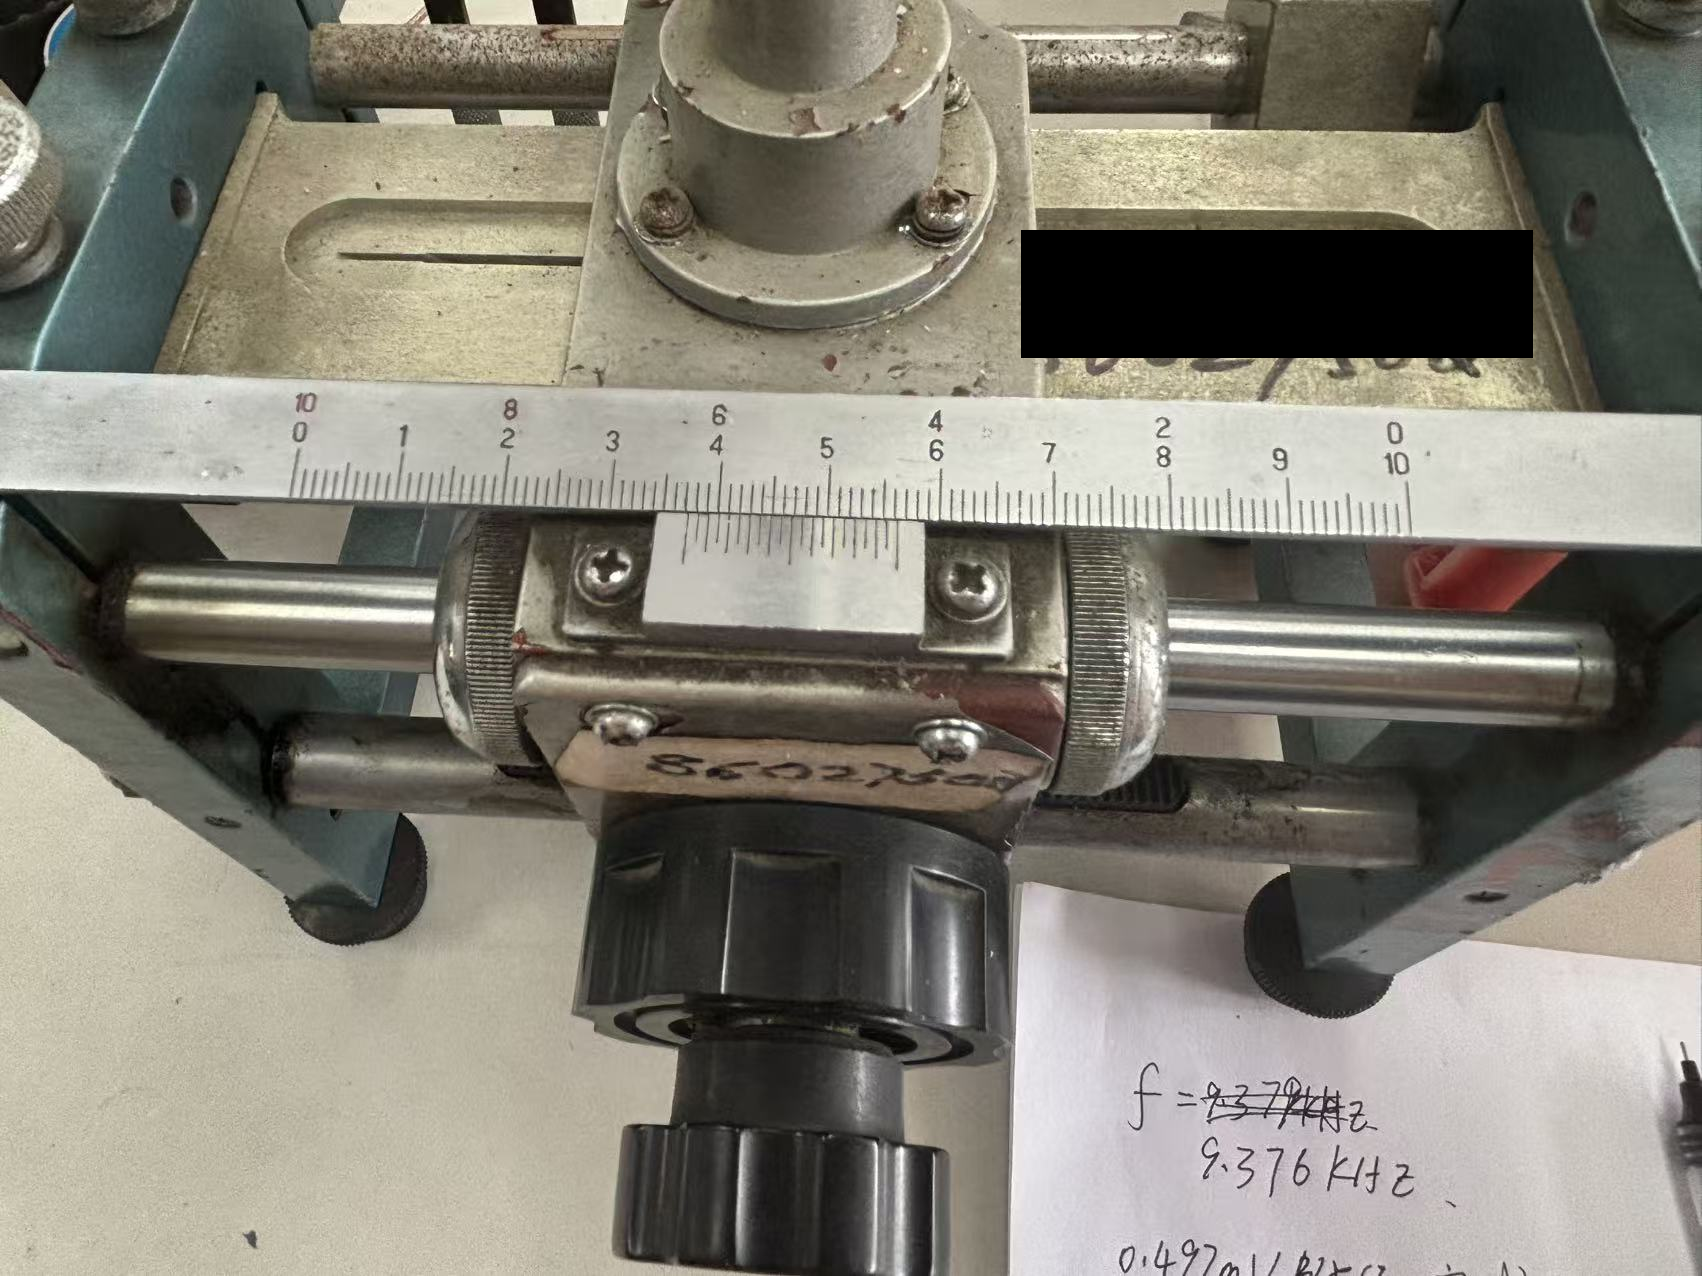
\includegraphics[width=\textwidth]{figures/node_position_1.png}
    \caption{第一个波节点}
  \end{subfigure}
  \begin{subfigure}{0.32\textwidth}
    \centering
    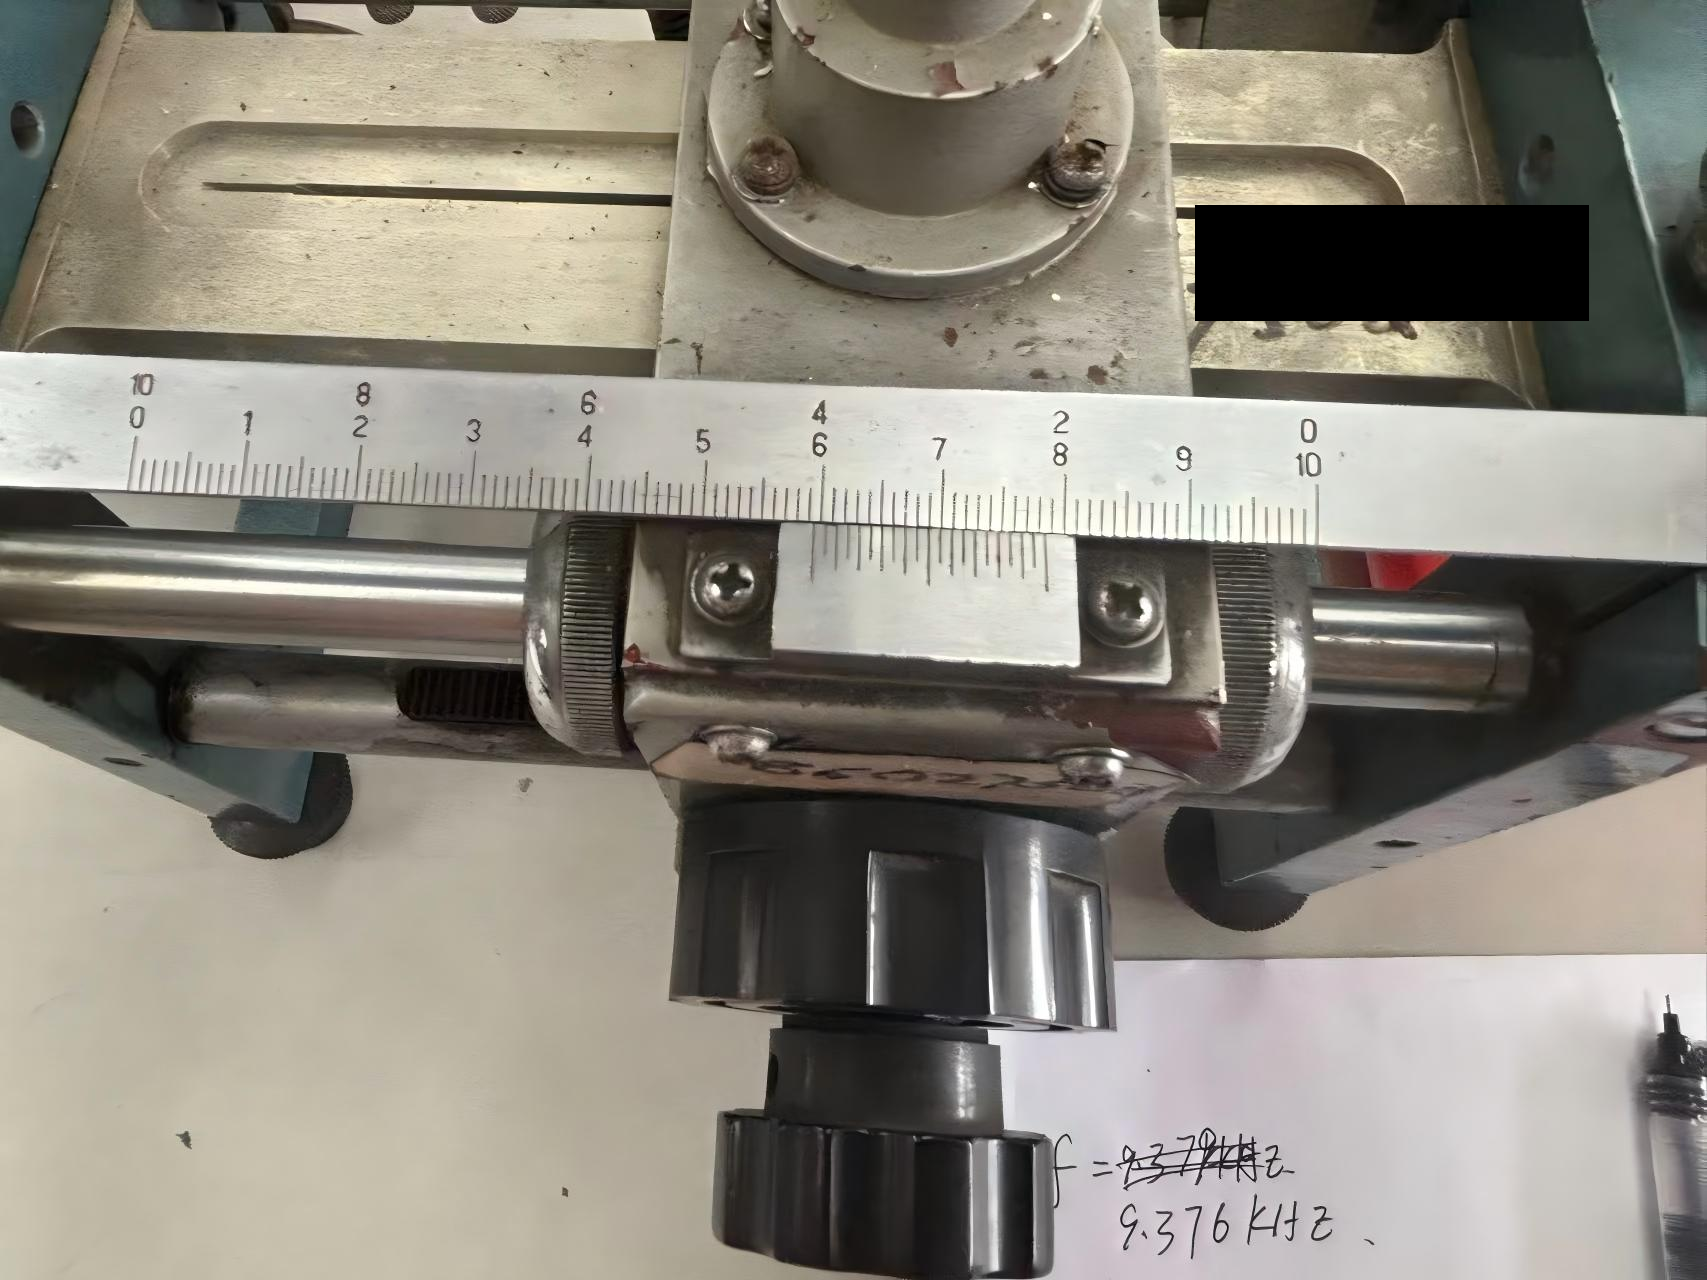
\includegraphics[width=\textwidth]{figures/node_position_2.png}
    \caption{第二个波节点}
  \end{subfigure}
  \caption{短路终端条件下的波导波长测量}
  \label{fig:wavelength-photo}
\end{figure}

\subsection{容性膜片负载测量}

为了确定负载驻波相位，先在短路块条件下记录等效短路波节点位置。之后拆下短路块，接入容性膜片和匹配负载，从短路参考位置附近向信号源方向寻找接入膜片后的第一个波节点，并继续移动探针寻找波腹位置，记录 $P_{\min}$ 与 $P_{\max}$。图 \ref{fig:capacitive-photo} 展示了容性膜片负载下的波节点和波腹读数。

\begin{figure}[H]
  \centering
  \begin{subfigure}{0.48\textwidth}
    \centering
    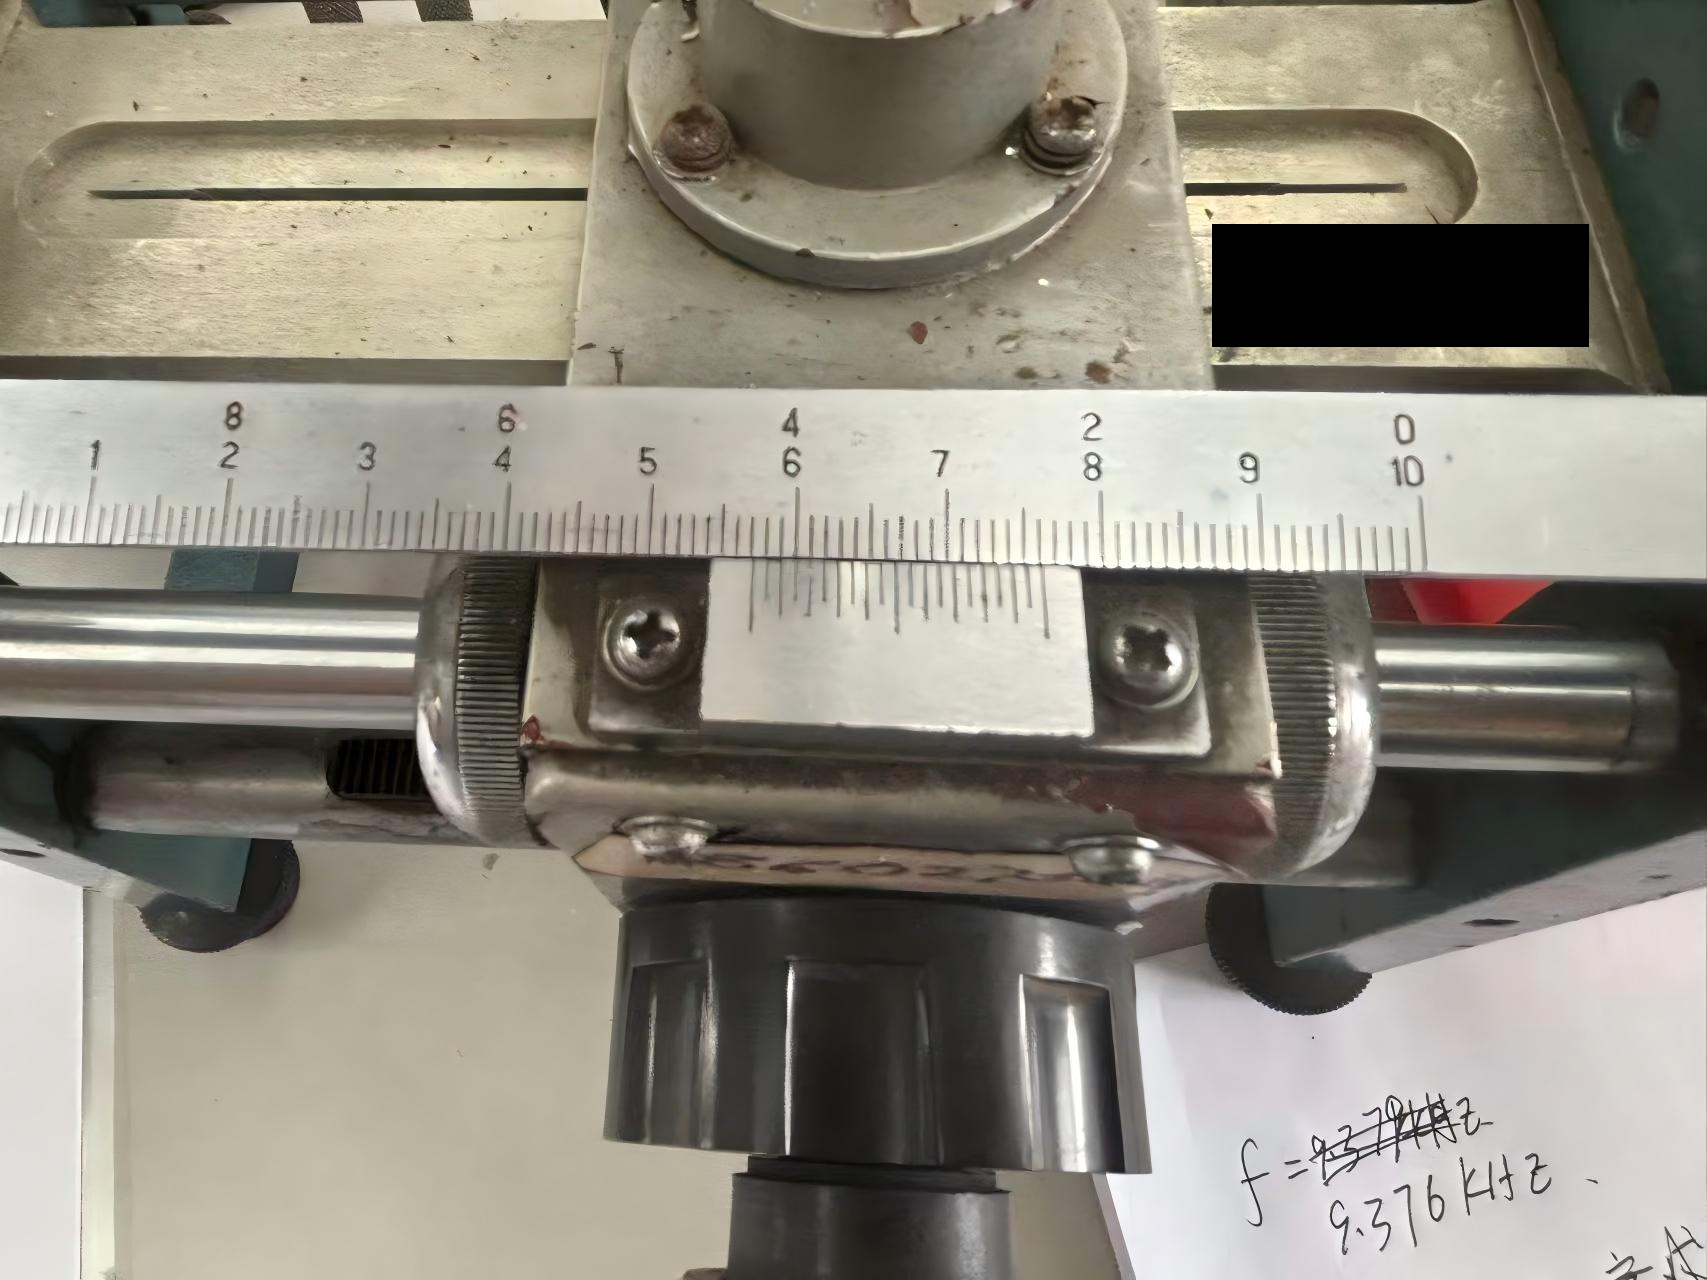
\includegraphics[width=\textwidth]{figures/capacitive_min.png}
    \caption{容性膜片负载波节点读数}
  \end{subfigure}
  \begin{subfigure}{0.48\textwidth}
    \centering
    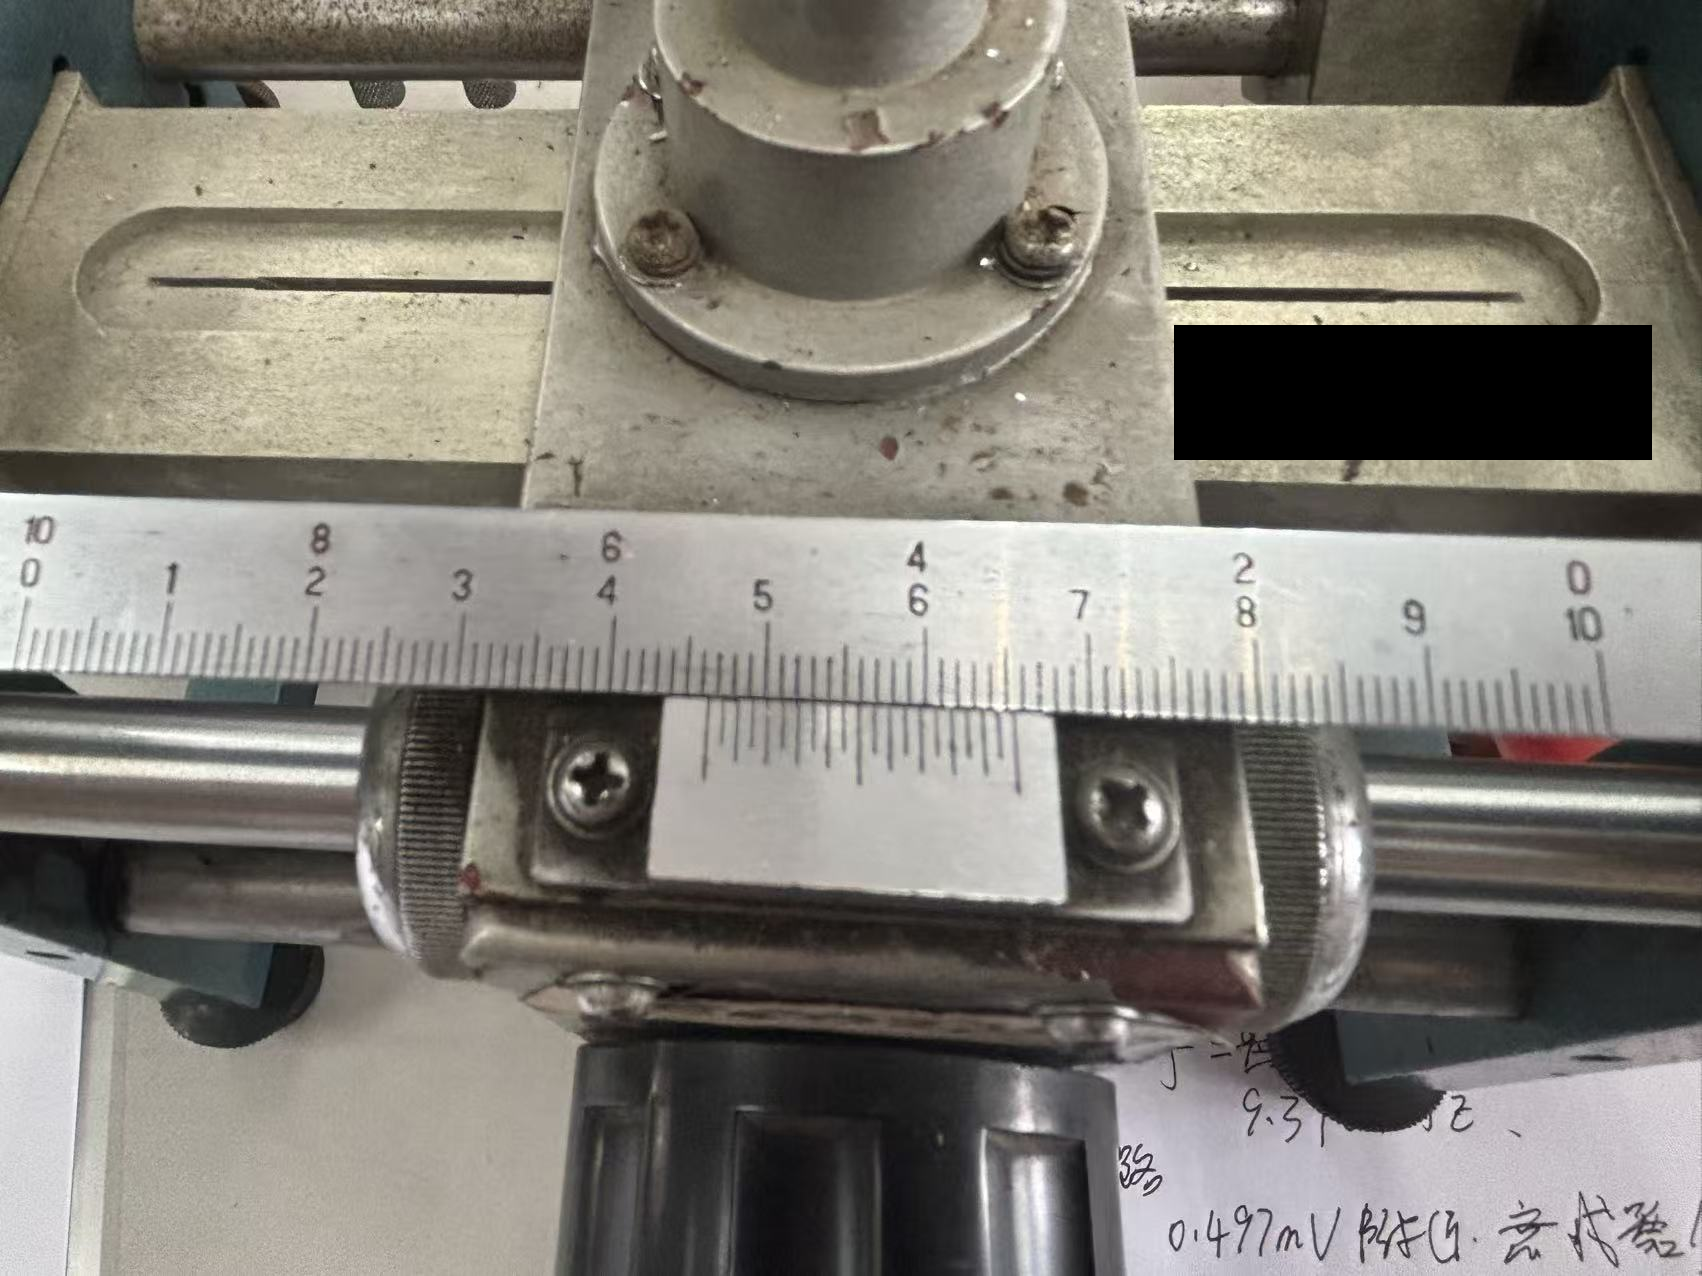
\includegraphics[width=\textwidth]{figures/capacitive_max.png}
    \caption{容性膜片负载波腹读数}
  \end{subfigure}
  \caption{容性膜片加匹配负载时的驻波测量}
  \label{fig:capacitive-photo}
\end{figure}

\subsection{单销钉匹配测量}

在驻波测量线和容性膜片负载之间接入单销钉调配器。先调节可调衰减器，使示波器上有足够的反射检波信号；再交替调节销钉纵向位置和插入深度，使定向耦合器采样到的反射信号尽可能减小。找到较佳匹配后，重新沿驻波测量线寻找最大和最小读数。最后拆去容性膜片，直接接入匹配负载，记录同等测量方法下的驻波读数，用作对照。相关照片见图 \ref{fig:match-photo}。

\begin{figure}[H]
  \centering
  \begin{subfigure}{0.32\textwidth}
    \centering
    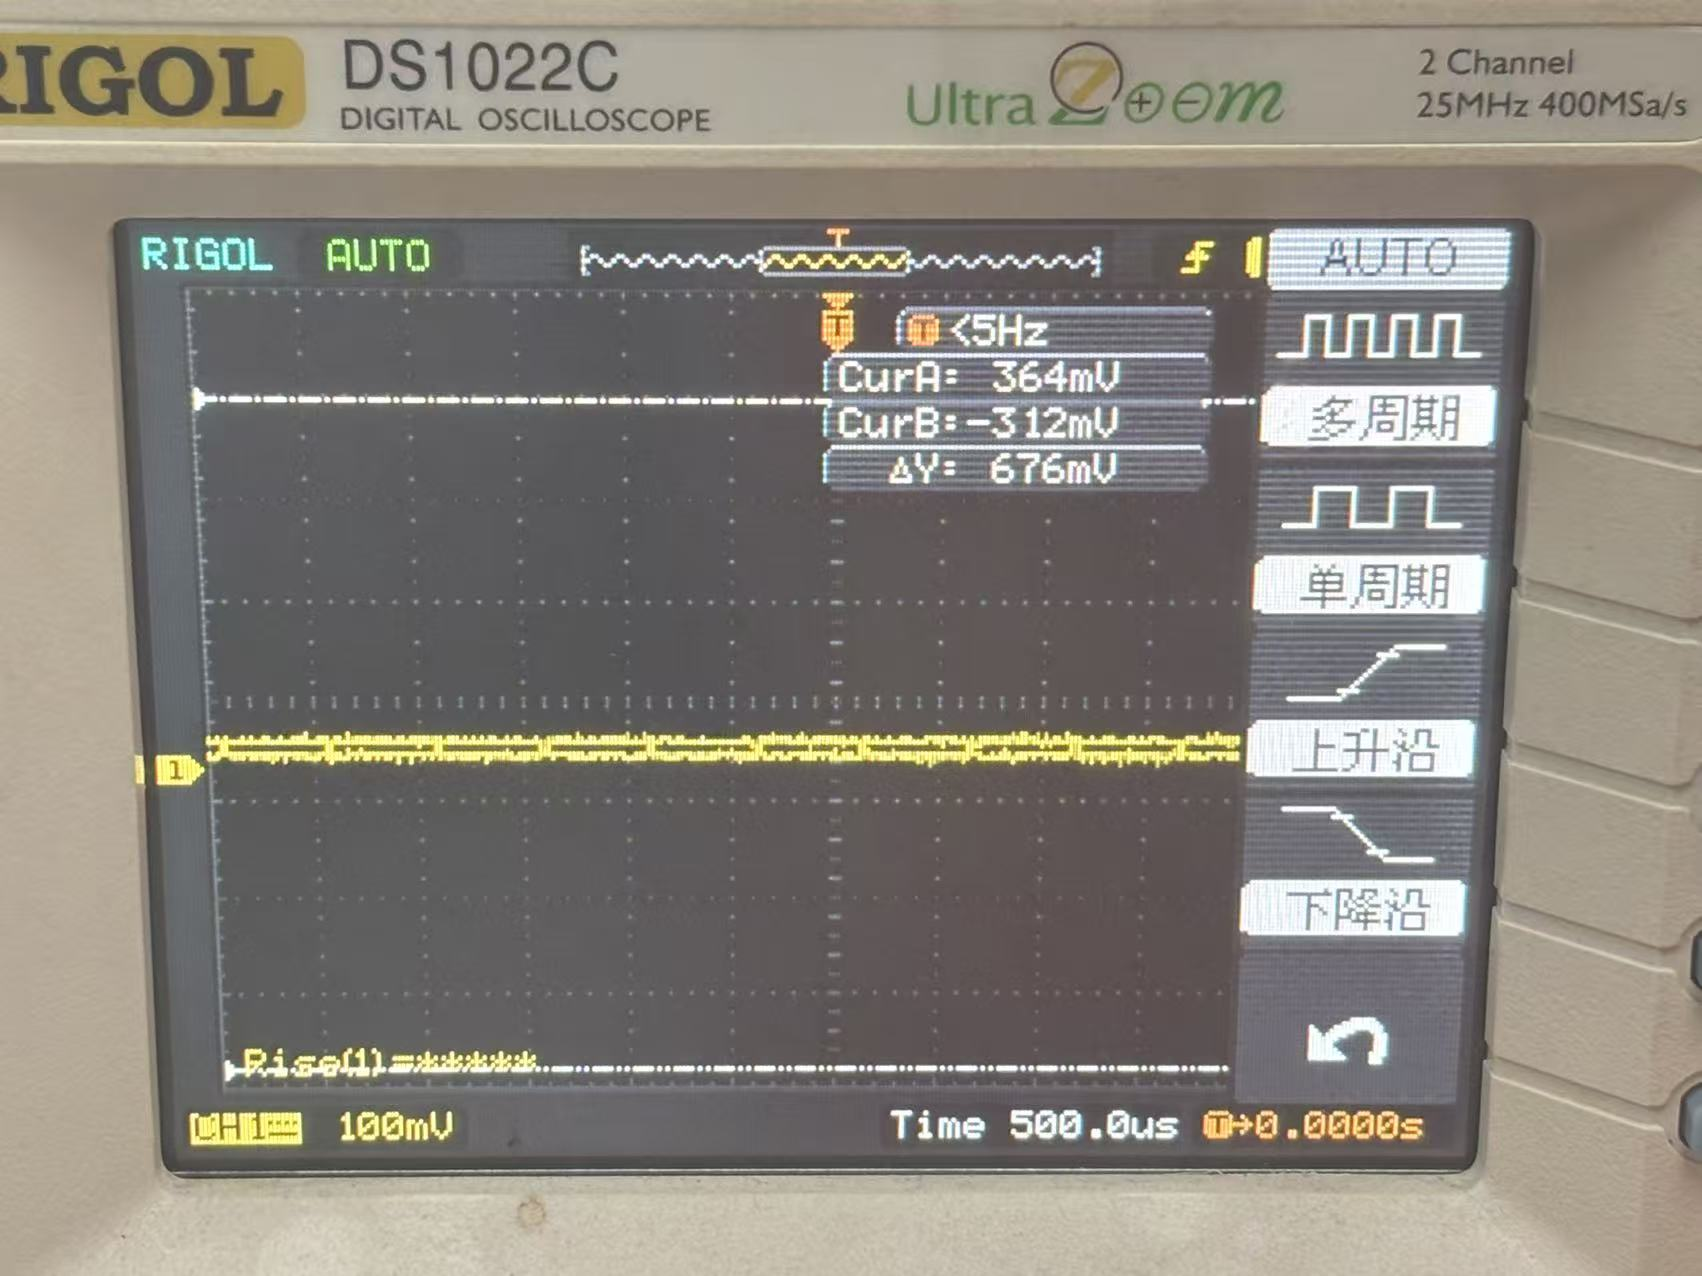
\includegraphics[width=\textwidth]{figures/pin_tuning_min.png}
    \caption{销钉调配反射最小}
  \end{subfigure}
  \begin{subfigure}{0.32\textwidth}
    \centering
    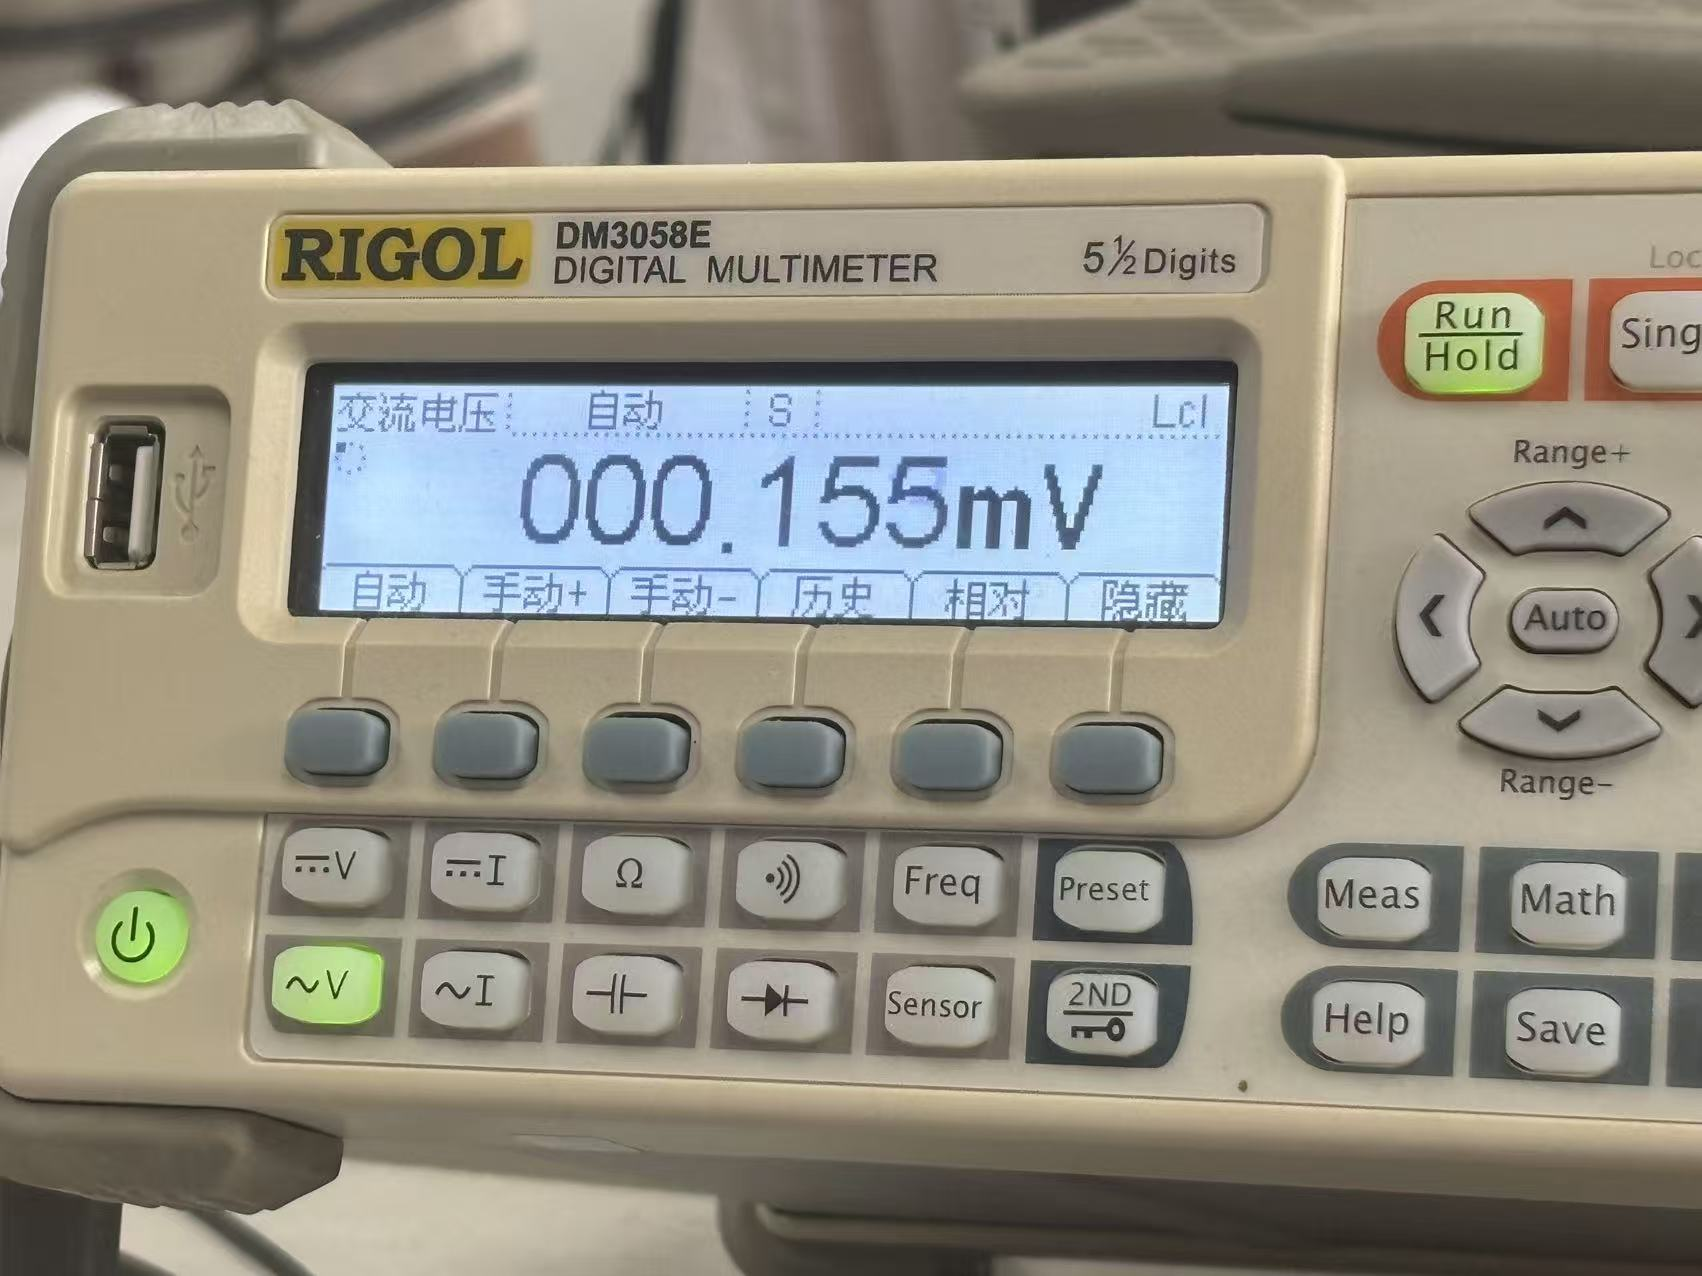
\includegraphics[width=\textwidth]{figures/pin_min.png}
    \caption{匹配后波节点}
  \end{subfigure}
  \begin{subfigure}{0.32\textwidth}
    \centering
    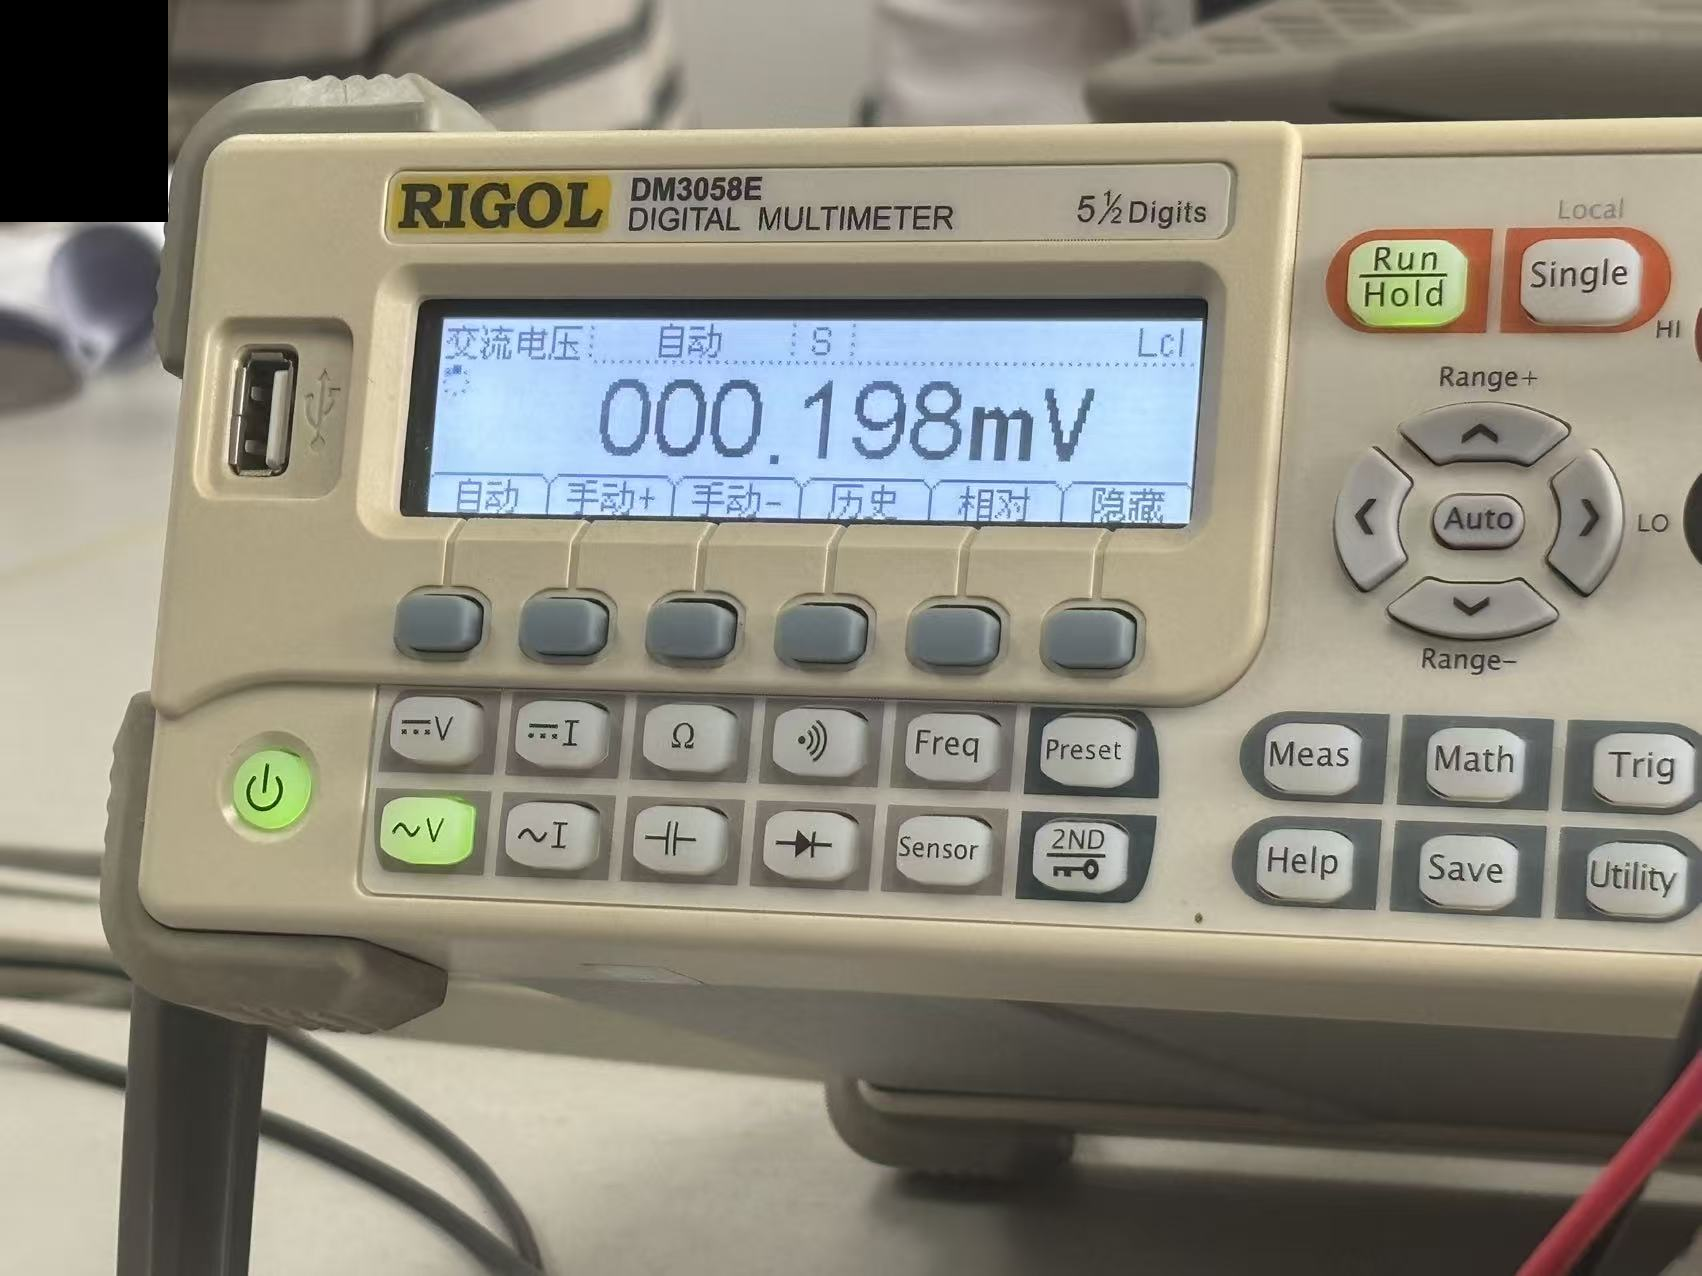
\includegraphics[width=\textwidth]{figures/pin_max.png}
    \caption{匹配后波腹}
  \end{subfigure}
  \caption{单销钉调配器匹配过程与驻波读数}
  \label{fig:match-photo}
\end{figure}

\begin{figure}[H]
  \centering
  \begin{subfigure}{0.48\textwidth}
    \centering
    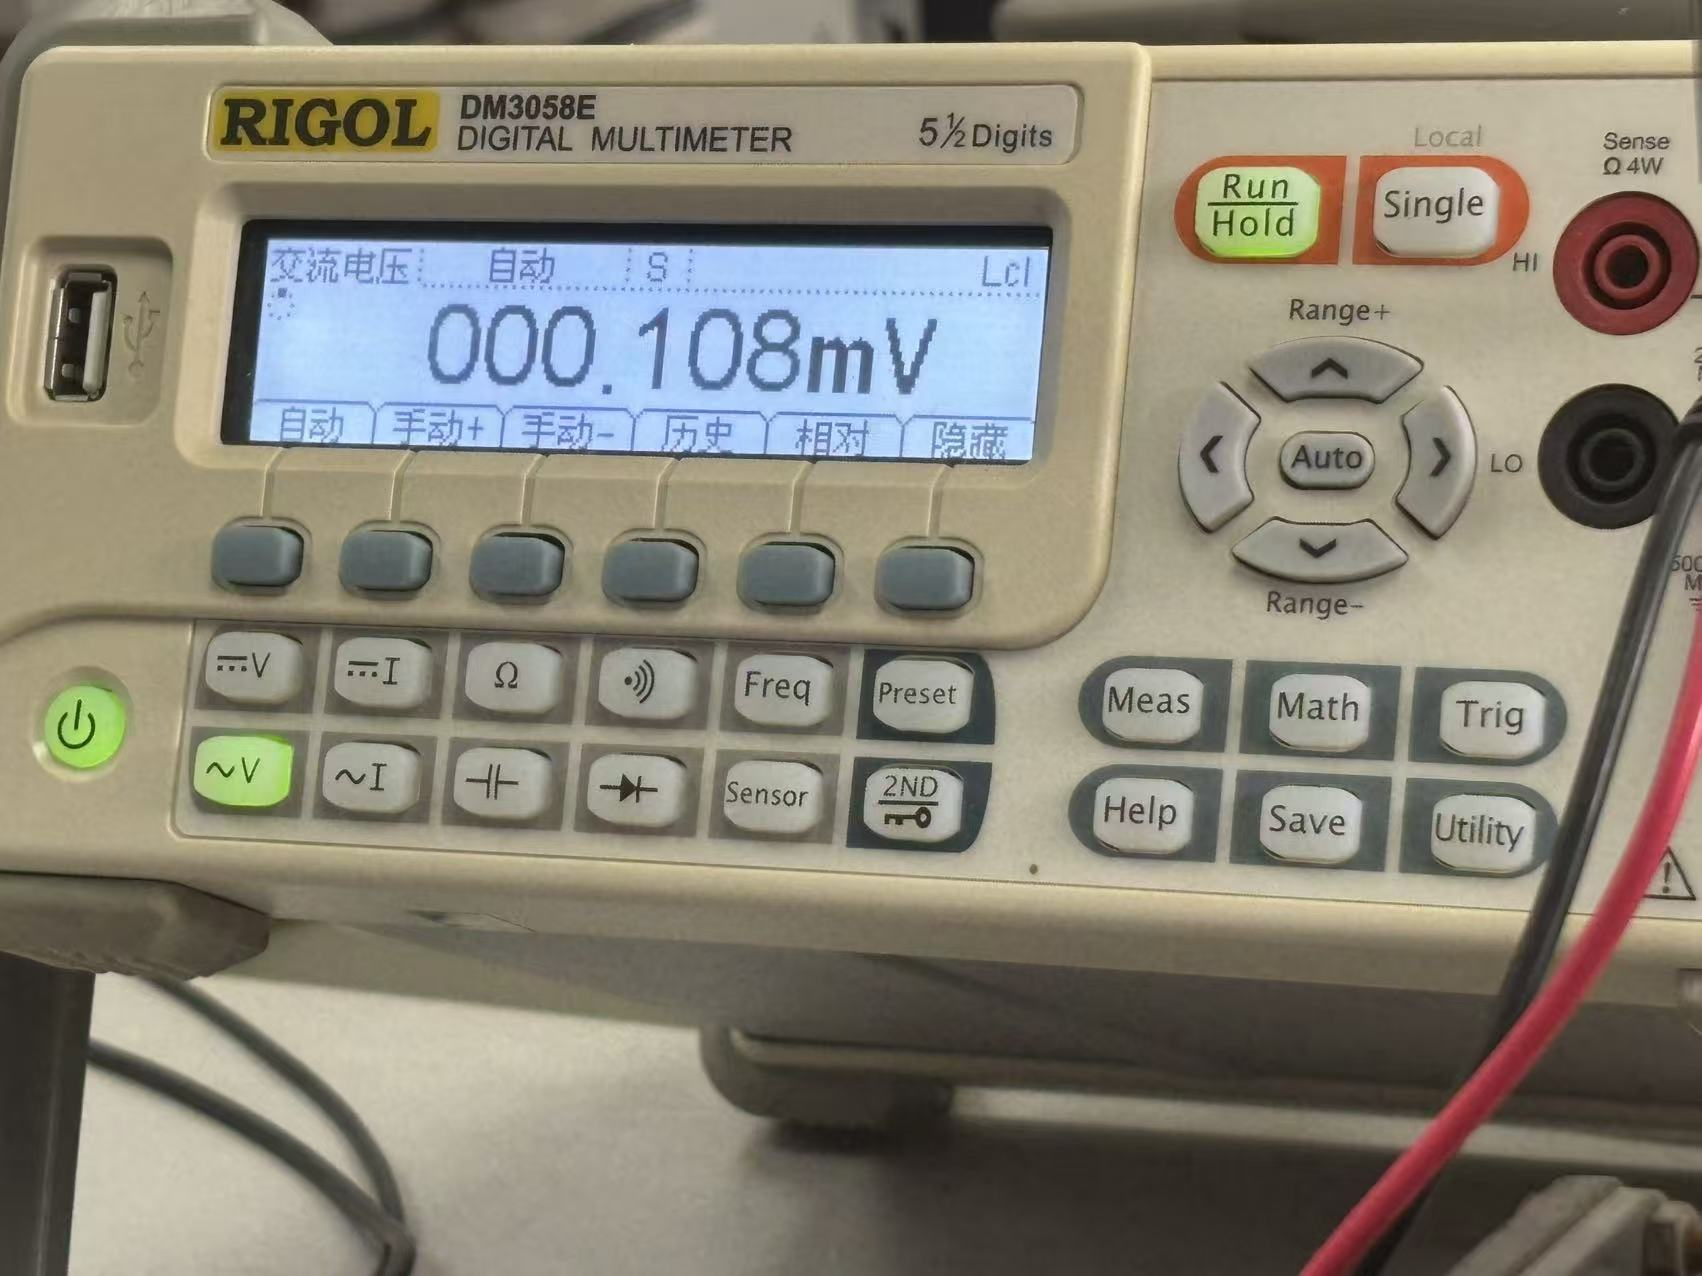
\includegraphics[width=\textwidth]{figures/matched_min.png}
    \caption{直接接匹配负载时的最小读数}
  \end{subfigure}
  \begin{subfigure}{0.48\textwidth}
    \centering
    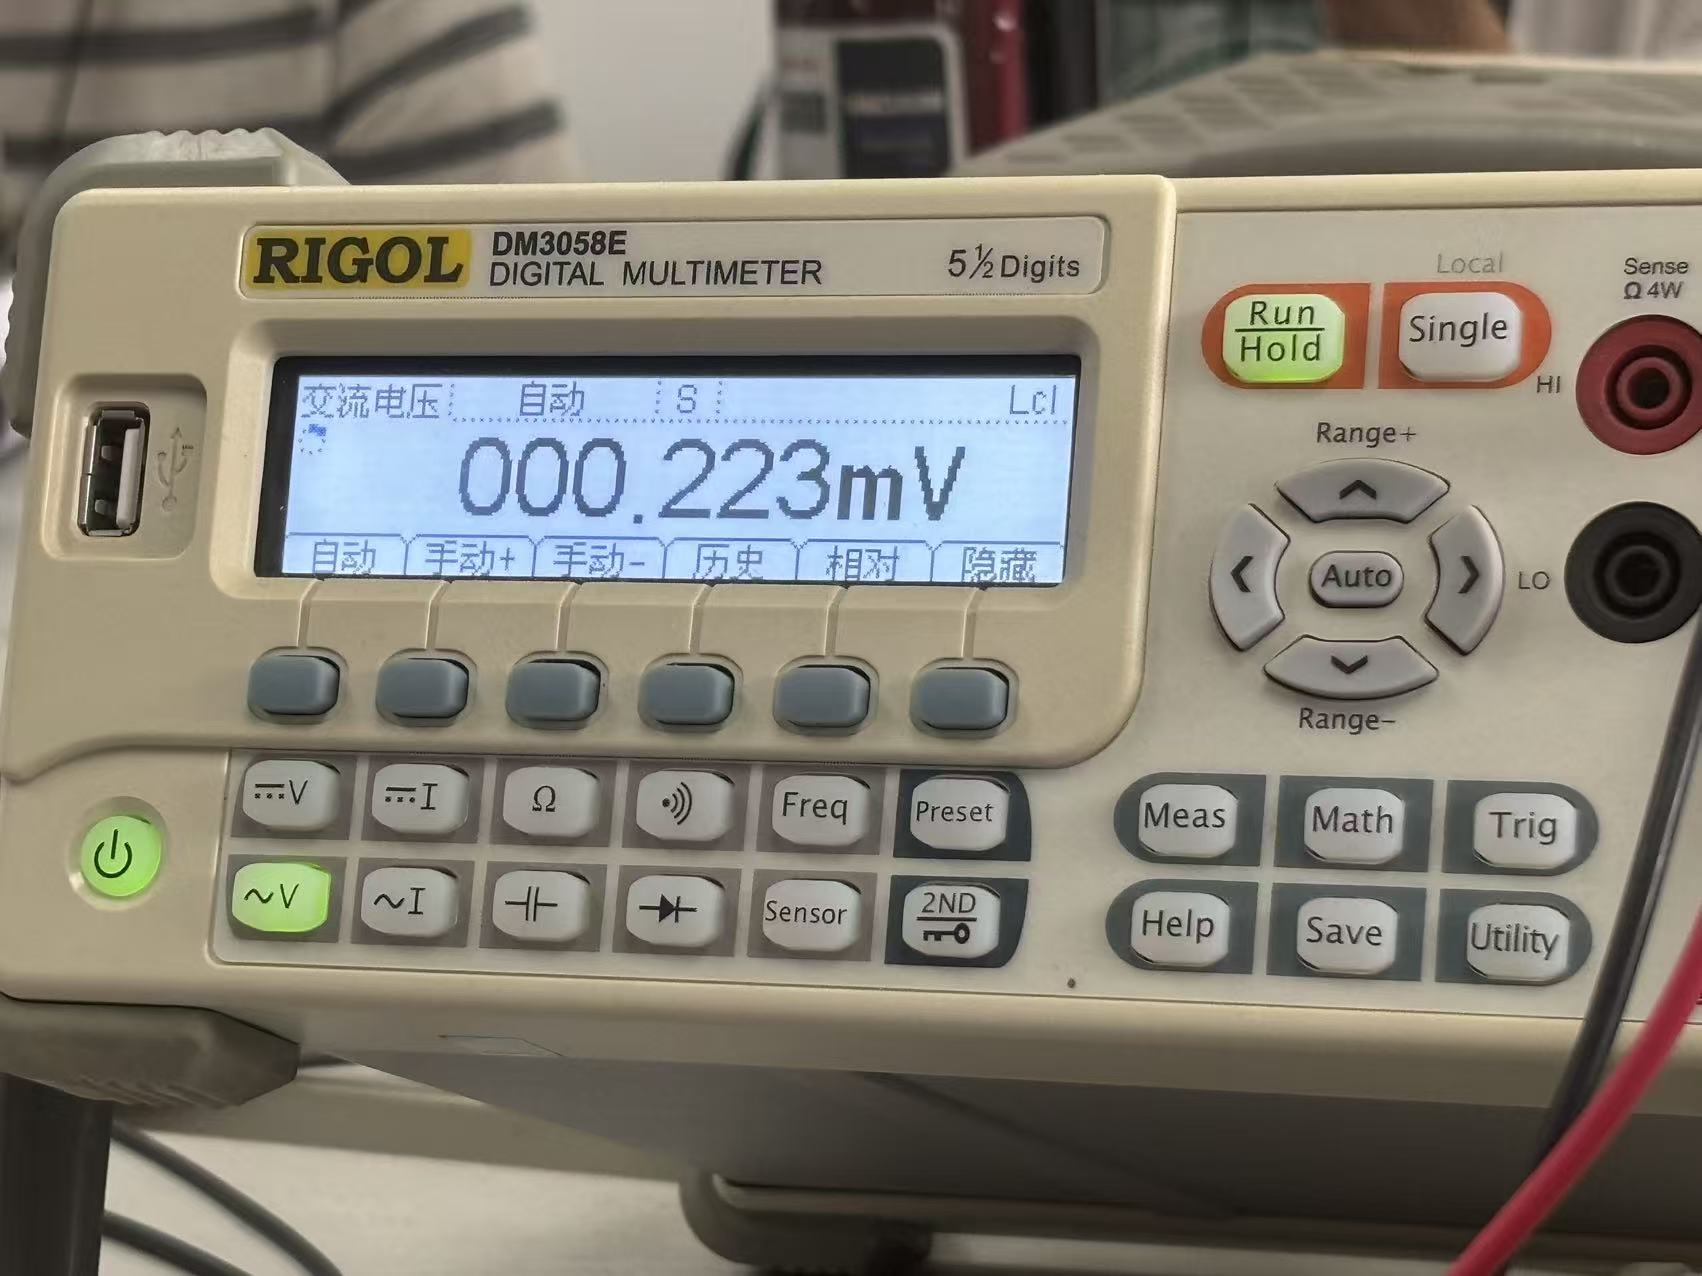
\includegraphics[width=\textwidth]{figures/matched_max.png}
    \caption{直接接匹配负载时的最大读数}
  \end{subfigure}
  \caption{匹配负载对照测量}
  \label{fig:matched-load-photo}
\end{figure}

\section{数据记录与处理}

\subsection{原始记录}

小组实验数据记录如图 \ref{fig:raw-record} 所示，整理后的关键数值列于表 \ref{tab:raw-data}。文中将数字万用表读数记为 $P$，单位仍按原始读数写为 $\mathrm{mV}$，但在驻波系数计算中只使用其相对比值。

\begin{figure}[H]
  \centering
  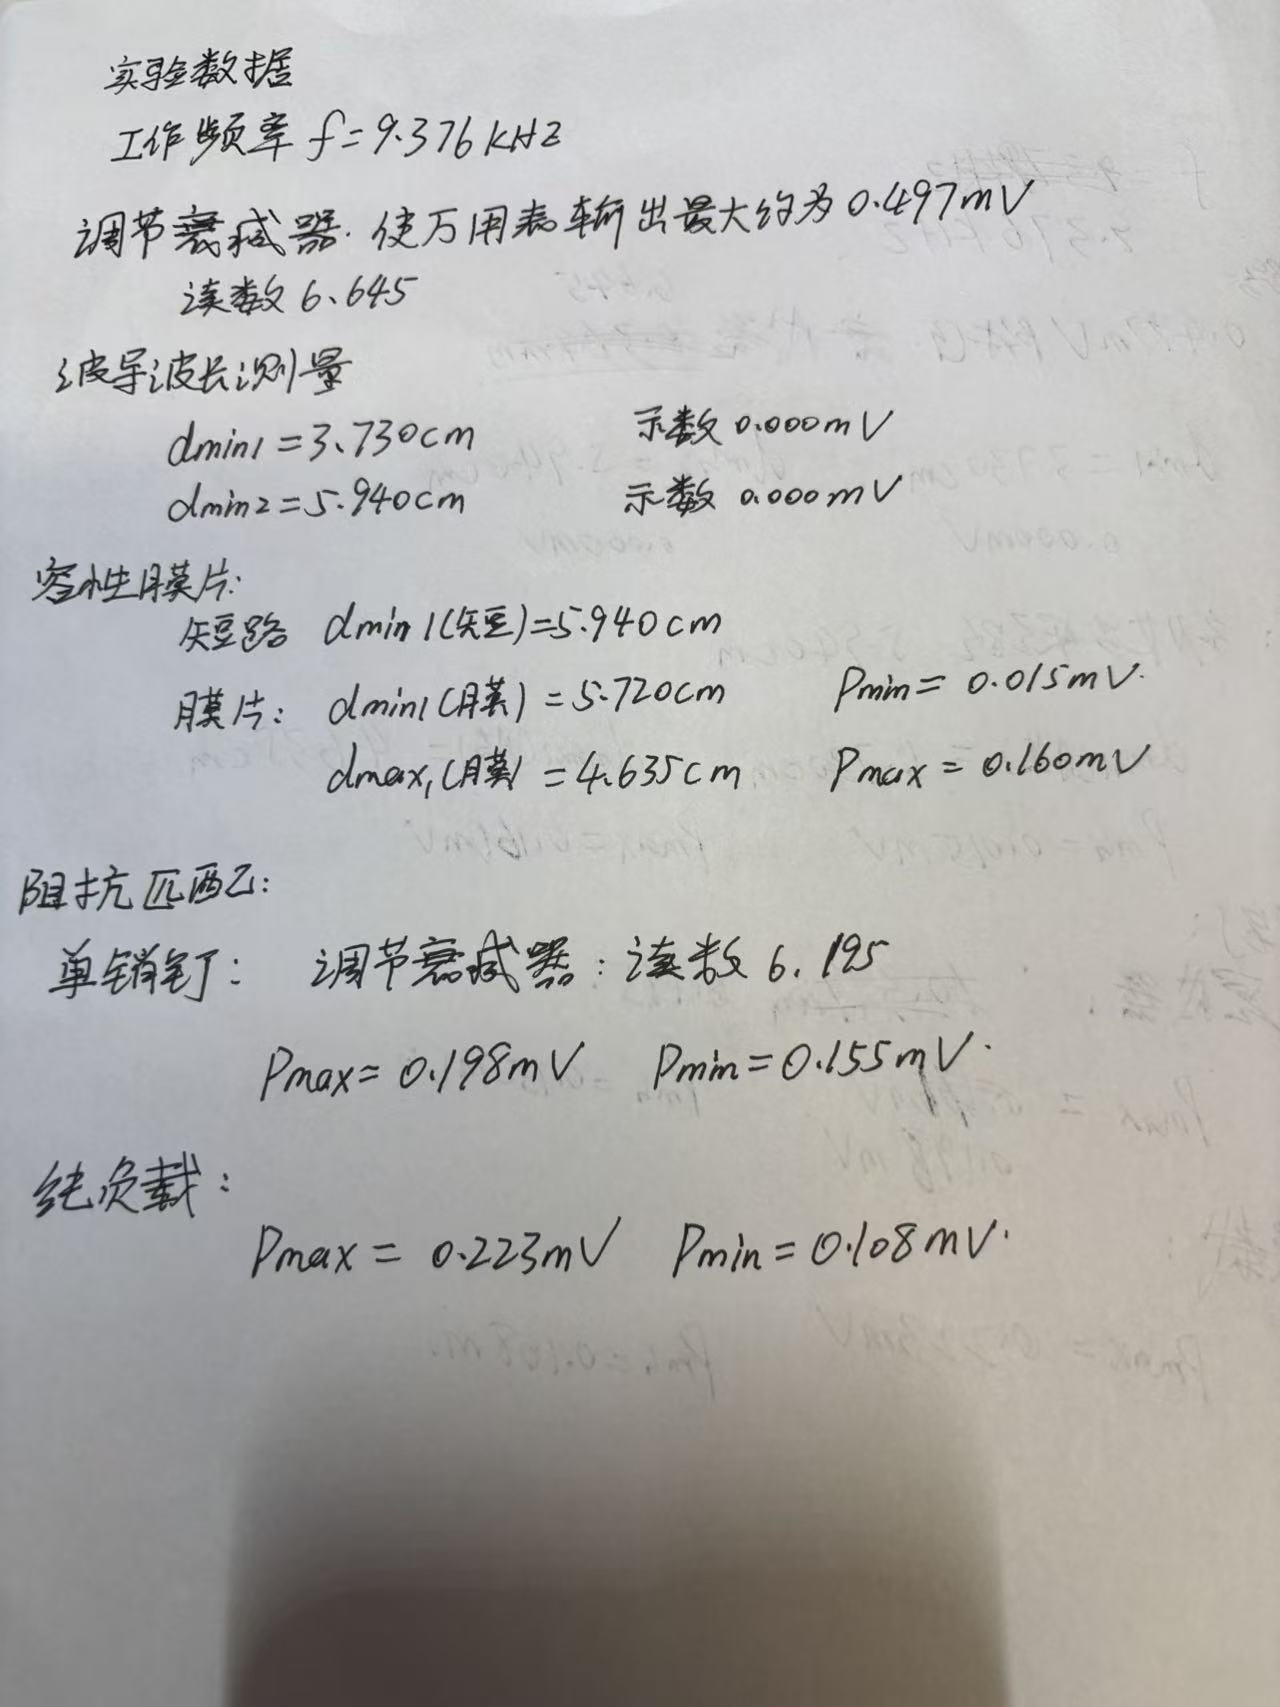
\includegraphics[width=0.72\textwidth]{figures/raw_data_record.png}
  \caption{本组实验数据原始记录照片}
  \label{fig:raw-record}
\end{figure}

\begin{table}[H]
  \centering
  \caption{实验原始数据整理}
  \label{tab:raw-data}
  \begin{tabular}{lll}
    \toprule
    项目 & 记录值 & 说明 \\
    \midrule
    工作频率 & $f=9.376\,\mathrm{GHz}$ & 直读式频率计读数 \\
    衰减器刻度 & $6.645$ & 波导波长测量前设置 \\
    短路波节点 1 & $d_{\min1}=3.730\,\mathrm{cm}$ & 万用表近似零读数 \\
    短路波节点 2 & $d_{\min2}=5.940\,\mathrm{cm}$ & 万用表近似零读数 \\
    容性膜片参考短路波节点 & $d_{\min}(\text{短})=5.940\,\mathrm{cm}$ & 等效短路面参考 \\
    容性膜片波节点 & $d_{\min}(\text{膜片})=5.720\,\mathrm{cm}$ & 负载接入后第一最小点 \\
    容性膜片波腹 & $d_{\max}(\text{膜片})=4.635\,\mathrm{cm}$ & 负载接入后最大点 \\
    容性膜片读数 & $P_{\min}=0.015\,\mathrm{mV}$，$P_{\max}=0.160\,\mathrm{mV}$ & 用于计算失配程度 \\
    单销钉匹配后 & $P_{\min}=0.155\,\mathrm{mV}$，$P_{\max}=0.198\,\mathrm{mV}$ & 销钉调配器接入 \\
    直接接匹配负载 & $P_{\min}=0.108\,\mathrm{mV}$，$P_{\max}=0.223\,\mathrm{mV}$ & 对照测量 \\
    销钉至负载距离 & $L=7.21\,\mathrm{cm}$ & 用于估算销钉电纳 \\
    \bottomrule
  \end{tabular}
\end{table}

后续数据处理依次完成实验指导书 1.4 中提出的要求：由实测波节点求 $\lambda_g$，计算 TE$_{10}$ 理论波导波长并比较，判读容性膜片负载的 $\Gamma$ 与 $z_L$，比较单销钉匹配和匹配负载两种驻波系数，并由销钉位置估算匹配状态下的归一化电纳/电抗。

\subsection{频率与波导波长的独立核算}

对波导波长的处理，我先把短路终端下的两个波节点看作同一驻波图样中的相邻最小点，而不使用负载测量阶段的数据。这样可以把波导色散参数和后续负载反算分开，避免一个测量误差同时进入两类结论。由 $d_{\min1}=3.730\,\mathrm{cm}$、$d_{\min2}=5.940\,\mathrm{cm}$ 得
\begin{equation}
  \lambda_{g,\mathrm{exp}}=2(5.940-3.730)=4.420\,\mathrm{cm}.
  \label{eq:lg-exp-num}
\end{equation}

以频率计读数 $f=9.376\,\mathrm{GHz}$ 为输入量，理论计算链列于表 \ref{tab:lambda-chain}。计算中统一使用厘米制，以便直接代入波导宽边 $a=2.286\,\mathrm{cm}$。

\begin{table}[H]
  \centering
  \caption{波导波长理论值与实测值核算}
  \label{tab:lambda-chain}
  \begin{tabular}{lll}
    \toprule
    处理量 & 计算式或取值 & 结果 \\
    \midrule
    自由空间波长 & $\lambda_0=c/f$ & $3.1974\,\mathrm{cm}$ \\
    TE$_{10}$ 截止波长 & $\lambda_c=2a$ & $4.572\,\mathrm{cm}$ \\
    理论波导波长 & $\lambda_0/\sqrt{1-(\lambda_0/\lambda_c)^2}$ & $4.4734\,\mathrm{cm}$ \\
    实测波导波长 & $2|d_{\min2}-d_{\min1}|$ & $4.4200\,\mathrm{cm}$ \\
    相对偏差 & $|\lambda_{g,\mathrm{exp}}-\lambda_{g,\mathrm{th}}|/\lambda_{g,\mathrm{th}}$ & $1.19\%$ \\
    \bottomrule
  \end{tabular}
\end{table}

这个偏差没有改变对传播模式的判断：若实际并非以 TE$_{10}$ 主模传播，波节点间距与式 \eqref{eq:lambdag-th} 给出的色散关系不会如此接近。因此，后续负载参数反算可以继续采用单模传输线模型。

\subsection{容性膜片负载的复反射系数}

容性膜片部分的原始读数包含两类信息：$P_{\max}/P_{\min}$ 决定反射系数幅值，波节点相对短路参考面的移动量决定相位。按照这个思路，先由平方律检波关系得到
\begin{equation}
  \rho_L=\sqrt{\frac{0.160}{0.015}}=3.266,\qquad
  |\Gamma_L|=\frac{\rho_L-1}{\rho_L+1}=0.5312.
\end{equation}
相位处理时采用短路波节点作为零相位参考。本组记录的两个位置为
\[
  d_{\min}(\text{膜片})=5.720\,\mathrm{cm},\qquad
  d_{\min}(\text{短})=5.940\,\mathrm{cm}.
\]
因此
\begin{equation}
  \Delta d=0.220\,\mathrm{cm},\qquad
  \varphi_L=4\pi\left(\frac{0.220}{4.420}-\frac{1}{4}\right)=-144.16^\circ.
\end{equation}
于是
\begin{equation}
  \Gamma_L=0.5312\angle(-144.16^\circ)
  =-0.4306-j0.3110.
\end{equation}

将该反射系数映射到阻抗平面和导纳平面：
\begin{equation}
  z_L=\frac{1+\Gamma_L}{1-\Gamma_L}=0.3349-j0.2902,
  \qquad
  y_L=\frac{1}{z_L}=1.7055+j1.4777.
  \label{eq:load-admittance}
\end{equation}
这里我更关注导纳形式，因为单销钉调配器在近似模型中是并联电纳。$y_L$ 的虚部为正，说明膜片主要引入容性电纳；$z_L$ 的实部小于 1，则说明该负载不只是纯电抗扰动，还改变了从参考面看入的等效有功导纳。

\subsection{Smith 圆图判读与计算互证}

实验要求在 Smith 圆图上读出容性膜片负载的反射系数和归一化阻抗。如图 \ref{fig:smith-load} 所示，$\Gamma_L=-0.4306-j0.3110$ 对应的点位于反射系数平面的第三象限，距圆心半径约为 $0.531$，落在 $\rho\approx3.27$ 的等驻波系数圆上。该点映射到阻抗圆图后处于下半平面，读得归一化阻抗约为 $z_L=0.3349-j0.2902$，说明膜片负载呈容性。

\begin{figure}[H]
  \centering
  \drawsmithchart
  \caption{容性膜片加匹配负载的 Smith 圆图位置与等驻波系数圆}
  \label{fig:smith-load}
\end{figure}

\begin{table}[H]
  \centering
  \caption{容性膜片负载的 Smith 圆图判读结果}
  \label{tab:smith-read}
  \begin{tabular}{lll}
    \toprule
    判读对象 & 结果 & 物理含义 \\
    \midrule
    反射系数位置 & $\Gamma_L=0.5312\angle(-144.16^\circ)$ & 强反射，且相位相对短路参考发生移动 \\
    归一化阻抗 & $z_L=0.3349-j0.2902$ & 阻抗实部偏小，虚部为容性 \\
    归一化导纳 & $y_L=1.7055+j1.4777$ & 并联容性电纳明显，适合用并联销钉补偿 \\
    驻波系数圆 & $\rho=3.266$ & 未调配时负载失配较强 \\
    \bottomrule
  \end{tabular}
\end{table}

这一判读也解释了为什么后续单销钉调配应优先在导纳圆图中理解：单销钉近似为并联支节，其作用不是改变负载本体，而是在某一截面加入一个可调电纳，把该截面的总导纳从 $1+jb$ 拉回到 $1+j0$。

\subsection{匹配前后的反射功率比较}

仅比较驻波系数容易低估匹配改善程度，因此我同时换算了反射功率比例 $|\Gamma|^2$ 和回波损耗。结果见表 \ref{tab:match-compare}。

\begin{table}[H]
  \centering
  \caption{三种负载状态的反射量化比较}
  \label{tab:match-compare}
  \begin{tabular}{lccccc}
    \toprule
    测量状态 & $\rho$ & $|\Gamma|$ & $|\Gamma|^2$ & $1-|\Gamma|^2$ & $RL$/dB \\
    \midrule
    容性膜片加匹配负载 & 3.266 & 0.5312 & 28.21\% & 71.79\% & 5.50 \\
    单销钉调配后 & 1.130 & 0.0611 & 0.374\% & 99.63\% & 24.27 \\
    直接接匹配负载 & 1.437 & 0.1793 & 3.215\% & 96.79\% & 14.93 \\
    \bottomrule
  \end{tabular}
\end{table}

从表中可见，单销钉调配后反射功率比例由 $28.21\%$ 下降到 $0.374\%$，约为原来的 $1/75.5$；回波损耗提高了 $18.77\,\mathrm{dB}$。这比只说“驻波系数接近 1”更能说明调配效果。值得注意的是，直接接匹配负载得到的 $\rho=1.437$ 反而差于单销钉调配后的结果。我的理解是，单销钉调配是在当前连接、当前膜片和当前测量线状态下做的就地补偿，而单独的匹配负载仍会受到法兰接触、负载频率特性和探针扰动影响，因此它在本次实测系统中不必然给出最小驻波。

\subsection{单销钉补偿电纳的核对}

销钉到负载的机械读数为 $L=7.21\,\mathrm{cm}$。导纳沿线每 $\lambda_g/2$ 重复，故可折算到
\begin{equation}
  l_\mathrm{eff}=7.21-3\times\frac{4.420}{2}=0.580\,\mathrm{cm}.
\end{equation}
把式 \eqref{eq:load-admittance} 的 $y_L$ 代入导纳变换式 \eqref{eq:y-transform}，在该截面得到
\begin{equation}
  y(l_\mathrm{eff})=0.984-j1.244.
\end{equation}
实部已经非常接近 1，因此它可以视为圆图上 $g=1$ 附近的调配点。若用数学条件 $\mathrm{Re}[y(l)]=1$ 反求最近位置，可得到 $l\approx0.576\,\mathrm{cm}$，与机械折算值只差约 $0.004\,\mathrm{cm}$，小于普通读数和销钉中心位置判断的不确定度。于是销钉应提供的并联电纳约为
\begin{equation}
  y_\mathrm{pin}\approx+j1.25,\qquad
  z_\mathrm{pin}\approx\frac{1}{j1.25}=-j0.80.
\end{equation}
图 \ref{fig:admittance-match} 用导纳圆图表示这一过程。负载导纳 $y_L$ 沿等驻波系数圆旋转到销钉所在截面后，已经接近 $g=1$ 圆；单销钉再提供约 $+j1.25$ 的并联电纳，将总导纳补偿到圆心附近。这说明单销钉并不是“消除负载本身的反射”，而是在它所在截面补上一个相反虚部，使源侧看到的总导纳接近 $1+j0$。

\begin{figure}[H]
  \centering
  \drawadmittancematchchart
  \caption{单销钉调配过程的导纳圆图说明}
  \label{fig:admittance-match}
\end{figure}

\subsection{容性膜片几何量与等效开口的附加估算}

实验指导书的鼓励内容要求进一步估算容性膜片的等效参数。小组记录中膜片开口高度和厚度约为
\[
  b'_\mathrm{geo}=4.0\,\mathrm{mm},\qquad d=1.0\,\mathrm{mm}.
\]
另一方面，也可以把实测负载导纳中的电纳 $B=1.4777$ 代入薄膜片近似公式，反推出一个“等效开口高度”。将 $B=1.4777$、$b=10.16\,\mathrm{mm}$、$d=1.0\,\mathrm{mm}$ 和
\[
  \beta'\approx\frac{2\pi}{44.20\,\mathrm{mm}}=0.1422\,\mathrm{rad/mm}
\]
代入
\begin{equation}
  b'^2+\frac{Bb}{\beta' d}b'-b^2=0
  \label{eq:bprime}
\end{equation}
得
\begin{equation}
  b'_\mathrm{eff}\approx0.97\,\mathrm{mm}.
\end{equation}
若把膜片近似成纯并联电纳，则其实测归一化容抗量级可写成
\begin{equation}
  x_{C,\mathrm{eq}}\approx-\frac{1}{B}=-0.677.
\end{equation}
该值与完整负载反算得到的 $z_L=0.3349-j0.2902$ 并不完全相同，因为后者包含了匹配负载、膜片损耗、参考面偏移以及传输线变换后的共同效果。$b'_\mathrm{eff}$ 明显小于几何开口 $4.0\,\mathrm{mm}$，说明薄膜片近似在本实验中更适合作定性比较：开口越窄，容性电纳越强；但要把它作为精确几何反推公式，则需要考虑有限厚度、边缘场和局部高次模。

\section{结果分析与误差讨论}

\subsection{实验结果的物理解释}

本实验最核心的现象可以概括为三步。第一，短路块使终端反射系数接近 1，因而驻波极小点清晰，测得的 $\lambda_g$ 与 TE$_{10}$ 理论值只差 $1.19\%$，支持了单模波导传输线模型。第二，容性膜片接入后，驻波系数升至 $3.266$，反射功率达到 $28.21\%$，说明负载与波导特性阻抗显著不匹配。第三，单销钉调配后反射功率降至 $0.374\%$，说明调配器在源侧实现了接近行波的状态。

容性膜片的特征不只体现在名称上，也体现在反算的导纳中：$y_L=1.7055+j1.4777$ 的正虚部对应并联容性电纳。若只看阻抗 $z_L=0.3349-j0.2902$，可以看到负电抗；若看导纳，则更容易和单销钉并联补偿过程连接起来。因此本报告在解释匹配机理时主要采用导纳圆图的思路。

\subsection{误差来源与影响方向}

\begin{enumerate}
  \item 波节点定位误差。波节点附近万用表读数变化慢，最小点位置容易受手动滑动和视差影响。若每个波节点按 $\pm0.01\,\mathrm{cm}$ 估计，则 $\lambda_g$ 的不确定度约为 $\pm0.028\,\mathrm{cm}$，已经达到理论与实测差值的一半量级。
  \item 检波平方律偏离。驻波系数通过 $\sqrt{P_{\max}/P_{\min}}$ 得到，要求检波器输出与功率成正比。若探针插入过深或输入信号过大，$P_{\max}/P_{\min}$ 会被非线性压缩或放大。
  \item 探针扰动。驻波测量线探针不是无扰动观察者，它会弱耦合能量并引入附加反射。调配前要求探针退出波导，正是为了避免把探针等效负载也一并匹配进去。
  \item 参考面不确定。短路块、容性膜片、单销钉和匹配负载都通过波导法兰连接，机械接触面并不一定就是电磁等效参考面。该误差主要影响反射系数相位和销钉距离折算。
  \item 器件非理想。匹配负载的实测 $\rho=1.437$ 表明它在本频点和本连接状态下并非理想 $1+j0$ 负载；这也解释了为什么就地调节的单销钉组合反而给出更低反射。
  \item 模型近似。理论处理默认只有 TE$_{10}$ 模、传输线无耗、膜片等效为集中并联电纳、销钉等效为纯电纳。实际膜片和销钉附近存在边缘场及局部高次模，这会使反算参数带有等效性。
\end{enumerate}

\section{思考题}

\subsection*{1. 测量线开口端不接短路块，任意接一负载，能否测出波导波长？接短路块有什么优点？}

能否测出波导波长，关键不在于负载是否一定为短路，而在于沿测量线能否形成足够清晰的驻波极小点。任意负载只要失配明显，都会产生反射，相邻两个电压最小点仍相隔 $\lambda_g/2$，因此原则上可以测出波导波长。但若负载接近匹配，线上场分布接近行波，$V_{\max}$ 与 $V_{\min}$ 差别很小，最小点位置会变得难以判定。

接短路块的优点是边界条件明确，反射系数幅值接近 1，驻波深度最大，波节点非常清楚；同时短路面还能提供稳定的相位参考。也就是说，短路测量不是唯一可行方法，但它是误差最小、判断最直观的方法。

\subsection*{2. 测负载驻波相位为什么要先测 $d_{\min}(\text{短})$？}

负载相位不是由某一个绝对刻度直接决定的，而是由负载接入前后驻波图样相对参考面的移动决定的。实际装置中，测量线刻度零点、法兰面、短路块的等效短路面并不严格重合。如果直接使用膜片负载的 $d_{\min}$，会把这些机械偏移误认为电磁相位。

先测 $d_{\min}(\text{短})$ 的作用，是在同一套连接和同一条测量线上建立相位零点。之后用 $d_{\min}(\text{膜片})$ 相对 $d_{\min}(\text{短})$ 的移动量求 $\varphi_L$，可以把共同的机械偏移抵消掉。这个步骤本质上是在做相位参考校准。

\subsection*{3. 在单销钉调配前，测量线探针为什么不能伸入到波导里面？}

驻波测量线探针虽然是测量部件，但它伸入波导后会耦合一部分能量，也会改变局部场分布。对主传输线来说，探针相当于一个额外的小负载，其大小与插入深度有关。

单销钉调配时希望补偿的是“容性膜片加匹配负载”本身。如果探针已经伸入波导，调配器看到的负载就变成“容性膜片、匹配负载、探针扰动”的组合。此时即使示波器上反射信号被调小，一旦改变探针深度，匹配状态也会被破坏。因此调配前应让探针退出或保持不扰动状态，调配完成后再用尽量浅的探针插入深度测量驻波。

\subsection*{4. 若改用感性膜片，驻波最小点会向信号源方向还是负载方向移动？}

本实验中容性膜片接入后，第一个驻波最小点相对短路参考点向信号源方向移动。感性膜片的等效电抗符号与容性膜片相反，因此反射系数相位相对短路参考的变化方向也相反。若保持同样的测量坐标和“寻找第一个最小点”的规则，感性膜片对应的驻波最小点应向负载方向移动。

从圆图角度看，容性负载和感性负载位于 Smith 圆图下、上两个不同半区。沿传输线移动时，阻抗点沿等驻波系数圆旋转；由于初始点在圆图上的半区相反，到达电压最小条件所需的相位位移也相反，所以最小点移动方向相反。

\subsection*{5. 单销钉调配时，为什么检波器输出指示越小表示调配越好？}

本实验的定向耦合器按反射功率取样方式连接，检波器输出主要对应从负载端返回信号源方向的波。单销钉调配的目标是让信号源侧看到的等效反射系数尽量小。

当销钉位置和插入深度逐渐合适时，负载反射波与销钉引入的反射补偿后，在输入侧合成的反射量减小。反射功率越小，经定向耦合器耦合到检波器的功率也越小，因此示波器或检波器指示越低，说明从源侧观察到的匹配越好。这里“越小越好”针对的是反射通道的检波信号，而不是传输到负载的有用功率。

\subsection*{6. 若经销钉调配后测得 $\rho=1$，单销钉调配器与负载之间是否是行波？单销钉至信号源方向是否是行波？}

若在单销钉调配器靠信号源一侧测得 $\rho=1$，只能说明该侧没有可观测的反射波，即单销钉调配器至信号源方向为行波状态。这个结论是“从输入端看进去匹配”，不是说整个负载系统内部处处匹配。

在单销钉调配器与容性膜片负载之间，负载本身仍然不是匹配负载，销钉本身也会产生局部散射。因此这一区间通常仍有入射波和反射波叠加，不能简单认为是行波。单销钉的作用更像是在某一截面加入合适电纳，使源侧总反射抵消为零；局部能量交换和局部驻波仍可能存在于销钉与负载之间。

\subsection*{7. 隔离器在系统中起什么作用？去掉隔离器会有什么影响？}

隔离器在系统中相当于微波源的“单向保护器”。它允许信号源输出的波向测量系统传播，同时把从负载端返回的反射波吸收在隔离端，减少反射波重新进入固态微波源。

如果去掉隔离器，负载失配产生的反射会直接反馈到信号源。这样一方面会改变源端等效负载，使输出幅度随负载调节而波动；另一方面可能牵引振荡频率，使频率计读数和驻波测量都不稳定。尤其在调单销钉和频率计时，系统反射状态不断变化，没有隔离器会使“被测对象变化”和“信号源状态变化”混在一起，增加判断难度。

\section{实验总结}

\begin{enumerate}
  \item 本实验测得微波系统工作频率为 $9.376\,\mathrm{GHz}$；由短路终端相邻波节点间距得到实测波导波长 $4.420\,\mathrm{cm}$。
  \item 根据矩形波导 TE$_{10}$ 模理论公式计算得到 $\lambda_{g,\mathrm{th}}=4.473\,\mathrm{cm}$，与实测值的相对误差为 $1.19\%$，说明实验系统主要按 TE$_{10}$ 模工作。
  \item 容性膜片加匹配负载的驻波系数为 $\rho=3.266$，反射系数为 $\Gamma=0.5312\angle(-144.16^\circ)$，归一化阻抗为 $z_L=0.3349-j0.2902$，归一化导纳为 $y_L=1.7055+j1.4777$。
  \item 经单销钉调配后，驻波系数降至 $1.130$，反射功率比例降至 $0.374\%$，表明单销钉调配器能够有效补偿容性膜片负载的电纳失配。
  \item 由销钉位置估算，匹配状态下销钉提供的归一化电纳约为 $+j1.25$，等效归一化阻抗约为 $-j0.80$。该结果与“沿线变换到 $g\approx1$ 后并联电纳补偿虚部”的 Smith 圆图匹配机理一致。
\end{enumerate}

\section{实验心得与体会}

本次实验让我把电磁场与电磁波课程中的若干抽象概念落到了具体测量对象上。课堂中讨论矩形波导 TE$_{10}$ 模时，波导波长、截止波长和相速度常以公式形式出现；在实验中，通过两个相邻波节点直接得到 $\lambda_g=4.420\,\mathrm{cm}$，再与理论值 $4.473\,\mathrm{cm}$ 比较，我对“波导中的波长不同于自由空间波长”这一点有了更直观的认识。它不是公式上的修正项，而是由边界条件和截止特性共同决定的传播结果。

我也更具体地理解了反射系数的相位意义。驻波系数只能说明反射强弱，不能唯一确定负载阻抗；只有加入波节点相对短路参考面的位移，才能把反射系数放到复平面上。这个过程把理论课中 $\Gamma=|\Gamma|e^{j\varphi}$ 的复数量，与实验中可移动探针读到的位置联系起来，使我意识到相位并不是附属量，而是阻抗测量中不可缺少的一半信息。

单销钉匹配部分加深了我对阻抗匹配的理解。调配后源侧驻波系数接近 1，并不意味着容性膜片本身变成了匹配负载，而是销钉和负载组成的新网络从输入端看近似匹配。也就是说，匹配可以通过在合适位置引入补偿电纳来实现；圆图中的“沿等驻波系数圆旋转”和“补偿虚部到圆心”，对应的正是传输线变换与并联支节调谐这两个物理过程。

此外，实验也提醒我微波测量对参考面和扰动非常敏感。探针插入深度、法兰接触状态、短路块等效面和隔离器都会影响结果。和低频电路相比，微波实验中的连接结构本身就是电路的一部分，不能简单忽略。这一点对理解后续高频系统、天线测量和微波网络参数都很重要。

\end{document}
